\documentclass[twoside,11pt]{article}

% Any additional packages needed should be included after jmlr2e.
% Note that jmlr2e.sty includes epsfig, amssymb, natbib and graphicx,
% and defines many common macros, such as 'proof' and 'example'.
%
% It also sets the bibliographystyle to plainnat; for more information on
% natbib citation styles, see the natbib documentation, a copy of which
% is archived at http://www.jmlr.org/format/natbib.pdf

\usepackage{jmlr2e}
\usepackage{multirow}

\usepackage{graphicx}
\usepackage{subfigure}
\usepackage{caption}
%\usepackage[colorlinks,citecolor=blue]{hyperref}


\usepackage{amsmath,amssymb}
\usepackage{amsthm}    % blackboard math symbols
\usepackage{bm}
\usepackage{mathtools}
\mathtoolsset{showonlyrefs}
\usepackage{enumitem}


\newtheoremstyle{definition}
  {.3em} % Space above
  {.1em} % Space below
  {} % Body font
  {} % Indent amount
  {\bfseries} % Theorem head font
  {.} % Punctuation after theorem head
  {.5em} % Space after theorem head
  {} % Theorem head spec (can be left empty, meaning `normal')


%\theoremstyle{plain}
\theoremstyle{definition}
\newtheorem{thm}{Theorem}
\newtheorem{lem}{Lemma}
\newtheorem{prop}{Proposition}
\newtheorem{pro}{Property}
\newtheorem{cor}{Corollary}
\newtheorem{defn}{Definition}
\newtheorem{assumption}{Assumption}
\newtheorem{example}{Example}
\newtheorem{rmk}{Remark}


\newtheorem{innercustomgeneric}{\customgenericname}
\providecommand{\customgenericname}{}
\newcommand{\newcustomtheorem}[2]{%
  \newenvironment{#1}[1]
  {%
   \renewcommand\customgenericname{#2}%
   \renewcommand\theinnercustomgeneric{##1}%
   \innercustomgeneric
  }
  {\endinnercustomgeneric}
}
\newcustomtheorem{customexample}{Example}


\newcommand*{\KeepStyleUnderBrace}[1]{%f
  \mathop{%
    \mathchoice
    {\underbrace{\displaystyle#1}}%
    {\underbrace{\textstyle#1}}%
    {\underbrace{\scriptstyle#1}}%
    {\underbrace{\scriptscriptstyle#1}}%
  }\limits
}
\allowdisplaybreaks
\usepackage{dsfont}


\usepackage{color}
\usepackage{algorithm}
\usepackage{natbib}
\usepackage{mathrsfs}

\usepackage{makecell}
\input macros.tex

\def\sign{\textup{sgn}}
\def\srank{\textup{srank}}
\def\rank{\textup{rank}}
\def\caliP{\mathscr{P}_{\textup{sgn}}}
\def\caliF{\mathscr{F}_{\textup{sgn}}}

\def\risk{\textup{Risk}}
\def\CPT{\text{\bf \footnotesize CPT}}
\def\NonParaM{\text{\bf \footnotesize NonparaM}}
\def\NonParaT{\text{\bf \footnotesize NonparaT}}

\usepackage[parfill]{parskip}

\usepackage{microtype}
\usepackage{xr}
\usepackage{algpseudocode}
\usepackage{booktabs}


\newcommand\Algphase[1]{%
\vspace*{-.7\baselineskip}\Statex\hspace*{\dimexpr-\algorithmicindent-2pt\relax}\rule{\textwidth}{0.4pt}%
\Statex\hspace*{-\algorithmicindent}\textbf{#1}%
\vspace*{-.7\baselineskip}\Statex\hspace*{\dimexpr-\algorithmicindent-2pt\relax}\rule{\textwidth}{0.4pt}%
}
\algnewcommand\algorithmicinput{\textbf{Input:}}
\algnewcommand\algorithmicoutput{\textbf{Output:}}
\algnewcommand\INPUT{\item[\algorithmicinput]}
\algnewcommand\OUTPUT{\item[\algorithmicoutput]}
% Definitions of handy macros can go here


% Heading arguments are {volume}{year}{pages}{submitted}{published}{author-full-names}

\jmlrheading{X}{20XX}{1-52}{6/2022}{XX/XX}{Chanwoo Lee and Miaoyan Wang}

% Short headings should be running head and authors last names

\ShortHeadings{Nonparametric tensor estimation}{Lee and Wang}
\firstpageno{1}


\raggedbottom
\begin{document}

\title{Beyond low-rankness: Nonparametric estimation and completion for sign-representable tensors}

\author{\name Chanwoo Lee  \email chanwoo.lee@wisc.edu \\
       \addr Department of Statistics\\
       University of Wisconsin-Madison
       \AND
       \name Miaoyan Wang \email miaoyan.wang@wisc.edu \\
       \addr Department of Statistics\\
       University of Wisconsin-Madison}

\editor{}

\maketitle

\begin{abstract}
Rapid developments in modern technologies have made tensor data readily available in daily life.
%We consider the problem of tensor estimation from noisy observations with possibly missing entries. 
Existing tensor estimation methods often rely on three assumptions: (i) a global low-rank structure across all tensor entries; (ii) a known, linear relationship between observed space and latent low-rank representation; (iii) separate treatments for tensors under various noise distributions. Here, we propose a nonparametric tensor estimation method based on a new model coined as \emph{sign representable tensors}. Our tensor model efficiently addresses possibly high-rank signals, allows various data types, and enjoys invariant property under unknown order-preserving entrywise transformations. We establish the excess risk bound, estimation error rate, and sample complexity for the tensor estimation problem with missingness. A key theoretical contribution is a provable reduction of complex (continuous) parameter estimation to a series of simpler (binary) sign estimations; this learning-reduction paradigm can be of independent interest. Further, we develop a divide-and-conquer algorithm to nonparametric tensor estimation with accuracy guarantees. We demonstrate the outperformance of our approach over previous methods on two datasets, one on human brain connectivity networks and the other on topic data mining. 
\end{abstract}

\begin{keywords}
tensor estimation, tensor completion, nonparametric statistics, weighted classification, rate of convergence, sample complexity.
\end{keywords}

\section{Introduction}\label{sec:intro}

%\footnotetext{Part of this work was presented at Advances in Neural Information Processing Systems Conference in December 2021 under the title ``Beyond the Signs: Nonparametric tensor completion via sign series''. However, this JMLR submission covers much deeper depth; many of the results have been substantially improved, sharpened, and expanded with new extensions. Therefore, this manuscript has limited overlap with the preliminary version.} 

\subsection{Motivation}\label{sec:motivation} 
Higher-order tensors have recently received much attention in enormous fields including social networks~\citep{anandkumar2014tensor}, neuroscience~\citep{zhang2019tensor}, and genomics~\citep{hore2016tensor}. Tensor methods provide effective representation of the hidden structure in multiway data. Our starting point is the signal plus noise model,
\begin{equation}\label{eq:modelintro}
\tY=\Theta+\tE, \quad \text{with}\quad \mathbb{E}(\tE)=0,
\end{equation}
where $\tY\in\mathbb{R}^{d_1\times \cdots \times d_K}$ is an order-$K$ data tensor, $\Theta$ is an unknown signal tensor of interest, and $\tE$ is a zero-mean noise tensor. Here, we take the convention that $\mathbb{E}(\cdot)$ is applied to the tensor $\tE$ in an entrywise fashion. The goal is to estimate $\Theta$ from the noisy observation $\tY$ with possibly missing entries. In particular, we focus on the following two problems:

\begin{itemize}[leftmargin=*,labelindent=-10pt]
\item[] Q1 (Nonparametric tensor estimation). How to accurately estimate $\Theta$ under a wide range of structures, including \emph{both low-rankness and high-rankness}?
\item[] Q2 (Complexity of tensor completion). How many observed tensor entries do we need to consistently estimate the signal $\Theta$ \emph{under a wide range of observation models}?
\end{itemize}

There is a huge literature on structured tensor estimation based on low-rankness of the signal tensor $\Theta$~\citep{jain2014provable,montanari2018spectral,anandkumar2014tensor,allen2012sparse} . Common low-rank models include Canonical Polyadic (CP) tensors~\citep{hitchcock1927expression}, Tucker tensors~\citep{de2000multilinear}, and block tensors~\citep{wang2019multiway}. Generalized linear tensor models~\citep{wang2018learning,hu2021generalized} are also proposed by assuming the low-rankness up to \emph{known} entrywise transformation.  
While these methods have shown great success in theory, tensors in applications often violate the low-rankness. Here we provide two examples to illustrate the limitation of classical low-rank models.

{\bf Sensitivity of tensor rank to transformation.} The first example reveals the sensitivity of tensor rank to order-preserving transformations. Let $\tZ \in \mathbb{R}^{30\times 30\times 30}$ be an order-3 tensor with tensor $\text{rank}(\tZ)=3$ (formal rank definition is deferred to the end of this section). Suppose a monotonic transformation $f(z)=(1+\exp(-cz))^{-1}$ is applied to $\tZ$ entrywise, and we let the signal $\Theta$ in model~\eqref{eq:modelintro} be the tensor after transformation. For illustration, we plot the numerical CP and Tucker rank of $\Theta$ versus $c$. The experiment details are provided in Appendix~\ref{sec:numericalrank}. Figure~\ref{fig:example}a shows that $\text{rank}(\Theta)$ far exceeds the intrinsic rank $\text{rank}(\tZ)=3$; in fact, the rank increases rapidly with the transformation level $c$. This observation suggests the failure of $\text{rank}(\Theta)$ in capturing the intrinsic model complexity. In practical applications of digital processing~\citep{ghadermarzy2018learning} and genomics analysis~\citep{hore2016tensor}, the tensor of interest often undergoes \emph{unknown} entrywise transformation prior to measurements. The rank sensitivity renders traditional low-rank tensor methods less desirable in the presence of even mild order-preserving nonlinearities. 

%The sensitivity to transformation makes the low-rank model less desirable in practice. 

\begin{figure}[h]
\centering
\includegraphics[width=\textwidth]{figure/example_ncomb.pdf}
\caption{(a) Numerical tensor rank (CP and Tucker) vs.\ transformation level $c$ in the first example. For Tucker rank, we plot the rank along first mode for illustration. (b) Top $d=30$ tensor singular values in the second example. The details of experiment are provided in Appendix~\ref{sec:numericalrank}.}
\label{fig:example}
\end{figure}


{\bf Limitation of low-rank family.} The second example demonstrates the inadequacy of classical low-rankness in representing special structures. Here we consider the signal tensor of the form $\Theta=\log(1+\tZ)$, where $\tZ\in\mathbb{R}^{d\times d\times d}$ is an order-3 tensor with entries $\tZ(i,j,k)=d^{-1}\max(i,j,k)$ for $i,j,k\in\{1,\ldots,d\}$. The matrix analogy of $\Theta$ was studied in graphon analysis~\citep{chan2014consistent}, and here we extend the structure to higher-order tensors. We find that neither $\Theta$ nor $\tZ$ is low-rank; in fact, Figure~\ref{fig:example}b
shows that all top $d$ tensor singular values are well above zero. Unlike matrices, tensor rank may even exceed the dimension $d$. This example shows the failure of classical low-rank models in capturing this type of tensor structures. 


In this paper, we develop a \emph{nonparametric tensor model} that efficiently addresses a wide range of tensor estimation problems. In the above and many other examples, the signal tensor $\Theta$ is possibly high rank. Classical low-rank models will miss important structures.  The observations have motivated us to develop a more flexible tensor estimation method. We will revisit these two motivating examples in Section~\ref{sec:common}, and show that our method overcomes the aforementioned limitations. 


\subsection{Our contributions}
We develop a nonparametric tensor model to address the aforementioned challenges. Existing tensor estimation methods often rely on three assumptions: (i) a global low-rank structure across all tensor entries; (ii) a known, linear relationship between observed space and latent low-rank representation; (iii) separate treatments for tensors under various noise distributions. By contrast, our proposed nonparametric model (i) enjoys rank invariance under monotonic transformations, (ii) allows both low-rank and high-rank effects, and (iii) provides a unified framework for both continuous and discrete data types.  
%Figure~\ref{fig:demo} illustrates our main idea. 

We highlight four main contributions that set our work apart from earlier literature. 


In modeling perspective, we present an innovative \emph{nonparametric} notion of complexity that incorporates more flexible structure than previously possible. Existing estimation theory~\citep{anandkumar2014tensor,montanari2018spectral,cai2019nonconvex} mostly focuses on the regime of low rank $r$ growing $d$. However, such premise fails in high-rank tensors, where the rank may grow with, or even exceed, the dimension. A proper notion of nonparametric complexity is crucial. Our key crux is built on the \emph{sign series representation} of the signal tensor, and we propose to estimate the sign tensors through a series of weighted classifications. In contrast to existing methods, our method is guaranteed to recover a wide range of low- and high-rank signals.  We show that, somewhat surprisingly, the sign tensor series not only preserves all information in the original signals, but also brings the benefits of flexibility and accuracy over classical low-rank models. The results fill the gap between parametric (low-rank) and nonparametric (high-rank) tensors, thereby greatly enriching the tensor model literature. 


In statistical perspective, we develop a  \emph{provable learning-reduction paradigm} by connecting the tensor estimation problem to a series of weighted classification tasks. This characterization converts a difficult $\mathbb{R}$-valued estimation problem, ``\emph{what} is the value of $\Theta$ at index $\omega$?'', to a series of relatively simpler $\{0,1\}$-valued problems, ``\emph{whether or not} the value of $\Theta$ at index $\omega$ falls below a threshold?'' We establish the excess risk bounds, estimation error rates, and sample complexity. 
As a by-product, the learning-reduction approach relaxes the common assumptions of homoscedastic normal noise; this flexibility provides a unified treatment for Gaussian, Bernoulli, and Binomial tensors. The result can be of independent interest for general nonparametric problems. 
%Our statistical guarantees not only improve the previous results for many well-studied tensor models but also reveals the rates that were previous impossible.
Considering the incisive minds that have studied tensor completion and nonparametric problems separately, our paper provides such connections that were not previously formulated.
 

In computational perspective, a number of efficient algorithms are readily available for $\{0,1\}$-valued tensor problems~\citep{wang2018learning, han2020optimal, ghadermarzy2018learning}. These algorithms enjoy computational efficiency while being restricted to binary inputs. Our work is orthogonal to these algorithm development, and we show that the high-rank tensor estimate is provably reducible to a series of binary tensor problems with carefully-designed weights. %This reduction provides a generic engine to empower existing algorithms for a wider range of structured tensor problems.
We develop a divide-and-concur approach to efficiently combine existing algorithms, thereby achieving computational accuracy without the need to reinvent the wheel. The flexibility to import and adapt existing algorithms is one advantage of our method. 

In application perspective, we demonstrate the advantages of our method through simulations and data applications. We apply our method to two datasets, one on brain connectivity study and the other on topic data analysis. The result shows that our approach not only improves the accuracy over previous tensor methods but also shows the robustness to model misspecification. Our method will help the practitioners efficiently analyze tensor datasets in various areas. Toward this end, our have released the software package at CRAN\footnote{https://CRAN.R-project.org/package=TensorComplete}.


\subsection{Related work}
Our work is closely related to but also clearly distinctive from several lines of existing research. We review related literature for comparison.


{\bf High-rank matrix models.} High-rank matrix estimation has been extensively studied under graphon models~\citep{chatterjee2015matrix,zhang2017estimating}, nonlinear models~\citep{ganti2015matrix} and subspace clustering~\citep{pmlr-v70-ongie17a,fan2019online}. In particular, the recent work~\citep{lee2021nonparametric} proposes a general nonparametric framework to address a variety of matrix problems including regression and completion.
However, high-rank tensor problems are more challenging for at least two reasons: (i) the tensor rank often exceeds the dimension when order $K$ greater than two~\citep{anandkumar2017analyzing}; this is in sharp contrast to matrices ($K=2$); (ii) the lack of tensor analogy for Eckart-Young theorem~\citep{kolda2003counterexample} poses theoretical challenges to extend matrix SVD thresholding~\citep{chatterjee2015matrix,xu2018rates} to higher-order tensors. %We show that, applying matrix methods to higher-order tensors results in suboptimal estimates. 
A full exploitation of the higher-order structure is therefore needed; we address this challenge in the paper. 

{\bf Nonparametric tensor regression.}
 The goal of tensor regression problem is to relate high-dimensional tensor covariates to a scalar response. There have been recent developments of nonparametric methods for tensor regression problems. \cite{hao2019sparse} proposed the additive regression model that exploits the sparse and low-rank structure in the tensor by extending the usual spline basis function. \cite{zhou2020broadcasted} combined multiple broadcasting operation and low-rank scaling coefficients to introduce nonlinearity on tensor entries. However, their results rely on low-rankness of the tensor, which might be restrictive in applications. By contrast, our method applies to both low-rank and high-rank tensors. Additionally, one fundamental difference is our tensor estimation problem works with a single tensor observation while tensor regression problem works with multiple tensor samples and corresponding responses. As a result, our theoretical error bound is based on tensor dimension while that of  tensor regression is a function of the sample size. %We leave extension of our framework to nonparametric tensor regression as future research.

{\bf Graphon and hypergraphon.} Graphon is a measurable function representing the limit of a sequence of exchangeable random graphs/matrices \citep{klopp2017oracle,gao2015rate,chan2014consistent}. Similarly, hypergraphon \citep{zhao2015hypergraph,lovasz2012large} is introduced as a limiting function based on a sequence of $K$-uniform hypergraphs, in which edges can join $K$ vertices with $K\geq 3.$ A special case of our \emph{sign representable tensor model} is related to, but also distinctive from, general hypergraphons; see Section~\ref{sec:common} for details. Both our model and hypergraphon use functions to represent signal tensors. However, there are two remarkable differences. First, unlike the matrix case where graphon is represented as a bivariate function, general hypergraphons for order-$K$  tensors are known to be represented by $(2^K-1)$-variate function~\citep{zhao2015hypergraph}. Our sign series representation depends on
$K$ coordinates only, and in this sense, our model shares common ground with \emph{simple hypergraphons}~\citep{balasubramanian2021nonparametric}. Second, our functional representation uses deterministic design points, whereas simple hypergraphons use random design points. These two choices lead to a notable difference in the root-mean-square rate $\tilde\tO(d^{-(K-1)/3})$ (ours) versus.\ $\tO(d^{-1})$ (simple hypergraphon; \cite{balasubramanian2021nonparametric}) where $d$ is tensor dimension. 
We see that our model has a substantially faster rate than simple hypergraphon as tensor order $K\rightarrow\infty$. Further comparison will be provided in Sections~\ref{sec:identifiability} and~\ref{sec:error}.


\subsection{Notation and organization}
We use $\mathbb{R}$ for the set of real numbers, $\mathbb{N}=\{0,1,2,\ldots,\}$ for integers, and $\mathbb{N}_{+}=\{1,2,\ldots\}$ for non-negative integers. 
We use $\sign(\cdot)\colon \mathbb{R}\to\{-1,1\}$ to denote the sign function, where $\sign(y)=1$ if $y\geq 0$ and $-1$ otherwise. We allow univariate functions (such as $\sign(\cdot)$, expectation $\mathbb{E}(\cdot)$, function $f\colon \mathbb{R}\to\mathbb{R}$, etc) to be applied to tensors in an element-wise manner. We use $[n]=\{1,\ldots,n\}$ for $n$-set with $n\in\mathbb{N}_{+}$. We denote $a_n\lesssim b_n$ if $\lim_{n\to\infty} a_n/b_n\leq c$ for some constant $c>0$, and $a_n\asymp b_n$ if $c_1\leq \lim_{n\to \infty} a_n/b_n\leq c_2$ for some constants $c_1,c_2>0$. We use $\tO(\cdot)$ to denote the big-O notation, $\tilde \tO(\cdot)$ to denote the variant hiding logarithmic factors, and $\text{poly}(d)$ to denote the polynomial complexity in integer $d$. 

Let $\Theta\in\mathbb{R}^{d_1\times \cdots \times d_K}$ denote an order-$K$ $(d_1,\ldots,d_K)$-dimensional tensor, and $\Theta(\omega)\in\mathbb{R}$ denote the tensor entry indexed by $\omega \in[d_1]\times \cdots \times [d_K]$. Denote $d_{\max}=\max_{k\in[K]}d_k$. 
%An event $A$ is said to occur ``with very high probability'' if $\mathbb{P}(A)$ tends to 1 faster than any polynomial of tensor dimension $d:=\min_k d_k \to\infty$. 
The CP decomposition~\citep{hitchcock1927expression} is defined by
 \begin{equation}\label{eq:CP}
\Theta=\sum_{s=1}^r\lambda_s\ma^{(1)}_s\otimes\cdots\otimes \ma^{(K)}_s,
 \end{equation}
 where $\lambda_1\geq \cdots \geq \lambda_r>0$ are tensor singular values, $\ma^{(k)}_s\in\mathbb{R}^{d_k}$ are norm-1 tensor singular vectors, and $\otimes$ denotes the outer product of vectors. 
 The minimal $r\in\mathbb{N}_{+}$ for which~\eqref{eq:CP} holds is called the tensor CP rank, denoted $\text{rank}(\Theta)$. Occasionally, we also use tensor Tucker rank, defined by
 \[
 \text{Tucker-rank} (\Theta)=(r_1,\ldots,r_k),\quad \text{where}\quad r_k=\text{rank}(\text{Unfold}_k(\Theta))\quad \text{for all }k\in[K], 
 \]
 where $\text{Unfold}_k(\Theta)$ denotes the unfolding operation that reshapes the tensor along model $k$ into a matrix of size $d_k$-by-$\prod_{i\neq k}d_i$, and $\text{rank}(\text{Unfold}_k(\Theta))$ denotes the usual matrix rank. The tensor maximum norm is denoted $\mnorm{\Theta}=\max_{\omega}|\Theta(\omega)|$, and the the tensor Frobenius norm is denoted $\Fnorm{\Theta}=\sqrt{\sum_{\omega}\Theta^2(\omega)}$.  We use $\mathbf{1}$ to denote a vector with all entries 1; the dimension of the vector should be clear from the contexts. 
 
The rest of the paper is organized as follows. In Section~\ref{sec:overview}, we propose the sign representable signal tensor model and a range of noise models. Algebraic and statistical properties of sign representable tensor model are provided in Sections~\ref{sec:algebry} and Section~\ref{sec:stat}, respectively. Section~\ref{sec:estimation} presents the learning-reduction approach to estimation and the finite sample accuracy. Important applications and extensions are also provided. Simulation and two data applications are presented in Section~\ref{sec:simulation}. Section~\ref{sec:conclusion} concludes the paper with discussion. Proofs and details for experiments are deferred to Appendix. 


\section{Sign representable tensor model}\label{sec:overview}
Let $\tY$ be an order-$K$ $(d_1,\ldots,d_K)$-dimensional data tensor generated from the model
\begin{equation}\label{eq:model}
\tY=\Theta+\tE, \quad \mathbb{E}(\tE)=0,
\end{equation}
where $\Theta\in\mathbb{R}^{d_1\times \cdots \times d_K}$ is an unknown signal tensor of interest, and $\tE\in\mathbb{R}^{d_1\times \cdots \times d_k}$ is a noise tensor consisting of zero-mean, independent \emph{but not necessarily identically} distributed entries. The goal is to estimate $\Theta$ from $\tY$ with possibly missing entries. 

%\section{Oracle properties of sign representable tensors}\label{sec:representation}
In the following sections, we propose the \emph{sign representable model} for the signal tensor $\Theta$ and a range of noise models for $\tE$ in~\eqref{eq:model}. We will show that our model addresses both low- and high-rank signals, while encompassing important tensor models---including CP models, Tucker models, single index models, simple hypergraphons---as special cases. In addition, our noise model allows general mean-to-variance dependence, thereby providing a unified framework for analyzing Gaussian, Bernoulli, and Binomial tensors.  %We establish the algebraic and statistical properties of sign representable, which serves the foundation for our method. 

%\subsection{Sign-rank and sign tensor series}\label{sec:sign-rank}
\subsection{Signal tensor model}
We first develop the structure assumptions on $\Theta$ in~\eqref{eq:model}. Let $\Theta$ be the signal tensor of interest, and $\sign (\Theta)$ the corresponding sign pattern. The sign patterns induce an equivalence relationship between tensors. Two tensors are called \emph{sign equivalent}, denoted $\simeq$, if they have the same sign pattern. 
\begin{defn}[Sign-rank]
The sign-rank of a tensor $\Theta\in\mathbb{R}^{d_1\times \cdots \times d_K}$ is defined by the minimal rank among all tensors that share the same sign pattern as $\Theta$; i.e.,
\begin{equation}\label{eq:sign-rank}
\srank(\Theta) := \min \{\rank(\Theta')\colon  \Theta'\simeq \Theta,\ \Theta'\in\mathbb{R}^{d_1\times \cdots \times d_K}\}.
\end{equation}
\end{defn}
The concept of sign-rank is firstly introduced in combinatorics~\citep{cohn2013fast}, complexity theory~\citep{alon2016sign}, and quantum mechanics~\citep{de2003nondeterministic}. Here we exploit this notion for nonparametric tensor estimation. The sign equivalence $\simeq$ induces a quotient space in $\mathbb{R}^{d_1\times \cdots \times d_K}$. Note that the sign-rank concerns only the sign pattern but discards the magnitude information of $\Theta$. In particular, $\srank(\Theta)=\srank(\sign \Theta)$. 

We now propose that the signal tensor $\Theta$ in model~\eqref{eq:model} falls into a general tensor family, which we coin as ``sign representable tensors''.
\begin{defn}[Sign representable tensor model] 
%Fix a level $\pi\in[-1,1]$. A tensor $\Theta$ is called $(r,\pi)$-sign representable, if the tensor $(\Theta-\pi)$ has sign-rank bounded by $r$. A tensor $\Theta$ is called $r$-sign (globally) representable, if $\Theta$ is $(r,\pi)$-sign representable for all $\pi\in[-1,1]$. The collection $\{\sign(\Theta-\pi)\colon \pi \in[-1,1]\}$ is called the sign tensor series. 
%We use $\caliP(r)=\{\Theta\colon \max_{\pi\in[-1,1]}\srank(\Theta-\pi)\leq r\}$ to denote the $r$-sign representable tensor family.
We define the sign-$r$ representable tensor family by 
\begin{equation}\label{def:sign}
\caliP(r)=\{\Theta\colon \max_{\pi\in[-1,1]}\srank(\Theta-\pi)\leq r,\ \mnorm{\Theta}\leq 1\}.
\end{equation}
A tensor $\Theta$ is called \emph{sign-$r$ representable} if $\Theta\in \caliP(r)$. We call the collection of binary tensors $\{\sign(\Theta-\pi)\colon \pi \in[-1,1]\}$ the \emph{sign tensor series} corresponding to $\Theta$. In general, the norm bound $\mnorm{\Theta}\leq 1$ in~\eqref{def:sign} can be replaced by $\mnorm{\Theta}\leq L$, where $L \in\mathbb{R}_{+}$ is an arbitrary constant; we choose $L=1$ for notational simplicity. 
\end{defn}

\begin{rmk}[Comparison with classical low-rank family] Our sign representable tensor family improves the classical low-rank family. The notion of sign-$r$ representability concerns the \emph{local} structure of $\Theta$. If we interpret the tensor $\Theta$ as a function $\Theta: [d_1]\times \cdots \times [d_K]\mapsto [-1,1]$, then the constraint $\srank(\Theta-\pi)\leq r$ imposes local model structure at each $\pi$ in the function range $[-1,1]$. The shifted tensor $(\Theta-\pi)$ needs not to be low-rank itself; only its sign pattern matters. This structure relaxes the classical low-rank family, where a \emph{global} low-rankness is imposed across all entry values of $\Theta$. In Section~\ref{sec:common}, we will show that our proposed sign representable tensor family substantially enriches the classical low-rank family. In particular, both tensor examples in Section~\ref{sec:motivation} (see Figure~\ref{fig:example}) are incorporated in $\caliP(r)$ but not in low-rank family. 
\end{rmk}


\subsection{Noise tensor model}
We now describe our model for noise tensor $\tE$ in~\eqref{eq:model}. We require that the noise tensor entries follow independent zero-mean assumption $\mathbb{E}(\tE)=0$ but otherwise no other distribution assumptions. In particular, we allow heterogeneous noise such that the noise variance $\text{Var}(\tE(\omega))$ may depend on index $\omega$. Our model~\eqref{eq:model} therefore provides a unified framework for a wide range of data types, including Gaussian, Bernoulli, Binomial, and mixtures of them. For instance, our model~\eqref{eq:model} incorporates the probability tensor estimation problem where $\tY$ is a binary tensor with entries $\{0, 1\}$ from Bernoulli distribution. In such a case, $\Theta=\mathbb{E}(\tY)$ represents the probability tensor to be estimated, and the noise variance depends on the mean, $\text{Var}(\tE(\omega))=\Theta(\omega)(1-\Theta(\omega))$. 

We also allow missing data. Our observation is a possibly incomplete data tensor, denoted  $\tY_\Omega$, from~\eqref{eq:model}, where $\Omega\subset[d_1]\times\cdots\times[d_K]$ denotes the index set of observed entries. We consider a general model of $\Omega$ that allows both uniform and non-uniform samplings. Specifically, let $\Pi=\{p_\omega\}$ be an arbitrarily predefined probability distribution over the full index set with $\sum_{\omega\in[d_1]\times \cdots \times [d_K]}p_\omega=1$. Let $\omega\sim \Pi$ denote the sampling rule, meaning that $\omega$'s in $\Omega$ are i.i.d.\ draws with replacement from distribution $\Pi$. The goal is to estimate $\Theta$ from $Y_{\Omega}$. 
%Note that $\Theta$ is not necessarily low-rank. 

\subsection{Important examples}\label{sec:common}
We next show that the sign-$r$ representable tensor family is a general model that incorporates most important tensor models, including low-rank tensors, single index models, generalized linear tensor models, and structured tensors with repeating entries. 

\begin{example}[CP/Tucker low-rank models] The CP and Tucker low-rank tensors are two most popular tensor models~\citep{kolda2009tensor}. Let $\Theta$ be a low-rank tensor with CP rank $r$. We see that $\Theta$ belongs to the sign representable family; i.e., $\Theta\in\caliP(r+1)$ (the constant $1$ is due to $\rank(\Theta-\pi)\leq r+1$). Similar results hold for Tucker low-rank tensors $\Theta\in\caliP(r+1)$, where $r=\prod_kr_k$ with $r_k$ being the $k$-th mode Tucker rank of $\Theta$.  
\end{example} 
\begin{example}[Tensor block models (TBMs)] Tensor block model~\citep{wang2019multiway,chi2020provable} assumes a checkerboard structure among tensor entries under marginal index permutation. The signal tensor $\Theta$ takes at most $r$ distinct values, where $r$ is the total number of multiway blocks. Our model incorporates TBM because $\Theta \in \caliP(r)$. 
\end{example}

\begin{example}[Generalized linear models (GLMs)] Let $\tY$ be a binary tensor from a logistic model~\citep{wang2018learning} with mean $\Theta=\text{logit}(\tZ)$, where $\tZ$ is a latent low-rank tensor. Notice that $\Theta$ itself may be high-rank (see Figure~\ref{fig:example}a). By definition, $\Theta$ is a low-rank sign representable tensor. Same conclusion holds for general exponential-family models with a (known) link function~\citep{hong2020generalized}. 
\end{example}

\begin{example}[Single index models (SIMs)] Single index model is a flexible semiparametric model proposed in economics~\citep{robinson1988root} and high-dimensional statistics~\citep{balabdaoui2019least,ganti2017learning}. The SIM assumes the existence of a (unknown) monotonic function $g\colon \mathbb{R}\to \mathbb{R}$ such that $g(\Theta)$ has rank $r$. We see that $\Theta$ belongs to the sign representable family; i.e., $\Theta\in \caliP(r+1)$. 
\end{example}

\begin{example}[Structured tensors with repeating entries]\label{eq:example} Here we revisit the model introduced in Figure~\ref{fig:example}c of Section~\ref{sec:motivation}. Let $\Theta$ be an order-$K$ tensor with entries $\Theta(i_1,\ldots,i_K)=\log(1+\max_kx^{(k)}_{i_k})$, where $x^{(k)}_{i_k}$ are given numbers in $[0,1]$ for all $i_k\in[d_k], k\in[K]$. We conclude that $\Theta \in \caliP(2)$, because the sign tensor $\sign(\Theta-\pi)$ with an arbitrary $\pi\in(0,\ \log 2)$ is a block tensor with at most two blocks. 

Example~\ref{eq:example} extends to general tensors with entries $\Theta(i_1,\ldots,i_K)=g(\max_kx^{(k)}_{i_k})$, where $g(\cdot)$ is an arbitrary polynomial of degree $r$. In this case, $\Theta$ is a high-rank tensor with at most $d_{\max}$ distinct entries but we have $\Theta\in \caliP(2r)$; see Proposition~\ref{prop:repeat} in the next section. Same conclusion holds if the maximum in $g(\cdot)$ is replaced by the minimum. 
\end{example}


\section{Algebraic properties of sign representable tensors}\label{sec:algebry}
In this section, we present algebraic properties for sign representable tensors~\eqref{def:sign}. 
Like most tensor problems~\citep{hillar2013most}, determining the sign-rank is NP hard in the worst case~\citep{alon2016sign}. Fortunately, tensors arisen in applications often possess special structures that facilitate analysis. We find that the sign-rank is upper bounded by tensor rank. More generally, we show the following properties.

\begin{prop}[Relationship between sign-rank and usual rank]~\label{cor:monotonic} \hfill
\begin{enumerate}[label={2.\arabic*},wide, labelwidth=!, labelindent=0pt,itemsep=0ex,parsep=0ex,topsep=-7pt]
\item[(a)] [Upper bounds] $\max_{\pi\in[-1,1]}\srank(\Theta-\pi)\leq \rank(\Theta)+1$.
\item[(b)] [Invariance under monotonic transformation] If $\Theta \in \caliP(r)$, then $g(\Theta)/\mnorm{g(\Theta)}\in\caliP(r+1)$ for any strictly monotonic function $g\colon \mathbb{R}\to \mathbb{R}$.\item[(c)] [Broadness] For every order $K\geq 2$ and every dimension $d$, there exist tensors $\Theta\in\mathbb{R}^{d\times \cdots \times d}$ such that $\rank(\Theta)\geq d$ but $\srank(\Theta-\pi)\leq 2$ for all $\pi\in\mathbb{R}$.  
\end{enumerate}
\end{prop}

Proposition~\ref{cor:monotonic} highlights the advantages of using sign-rank in the high-dimensional tensor analysis. The property (a) implies that the classical low-rank family is a special case of our sign representable tensor family.  The property (b) shows that, compared to classical tensor rank, the sign-rank remains nearly invariant under monotonic transformations; this is because $\srank(g(\Theta))\leq 1+\srank(\Theta)$ for all strictly monotonic function $g$. The property (c) shows that the sign-rank can be dramatically smaller than the classical tensor rank. Therefore, our model family $\caliP(r)$ is strictly richer than the usual low-rank family. 
%In particular, the sign-rank can be much smaller than the tensor rank, as we have shown in the two examples of Section~\ref{sec:motivation}. We provide several additional examples below in which the tensor rank grows with dimension $d$ but the sign-rank remains a constant. 


%\subsection{More examples with high tensor rank but low sign-rank}\label{sec:high-rank}
In Section~\ref{sec:common}, we have provided several tensor examples with high tensor rank but low sign-rank. Here we provide additional examples in which the tensor rank grows with dimension but the sign-rank remains a constant. Important examples are generalized into related propositions. Proofs are deferred to Appendix~\ref{sec:proofalg}. For notational simplicity, we consider tensors of equal dimension at each mode; i.e., $d_1=d_2=\cdots=d_K=d$. 


\begin{example}[Structured tensors with repeating entries]\label{example:max} Suppose a tensor $\Theta$ takes the form 
\[
\Theta(i_1,\ldots,i_K)=\log\left(1+{1\over d}\max(i_1,\ldots,i_K)\right), \ \text{for all }(i_1,\ldots,i_K)\in[d]^K.
\]
 Then 
 \[
 \rank(\Theta)\geq d, \quad \text{and}\quad \srank(\Theta-\pi)\leq 2\ \text{for all }\pi\in\mathbb{R}. 
 \]
\end{example}
More generally, Examples~\ref{eq:example}-\ref{example:max} are special cases of the following proposition. 

\begin{prop}[Rank relations for structured tensors with repeating entries]\label{prop:repeat}Let $g\colon \mathbb{R}\to \mathbb{R}$ be a continuous function such that $g(z)=0$ has at most $r\geq 1$ distinct real roots. For given numbers $x^{(k)}_{i_k}\in[0,1]$ with $i_k\in[d_k]$, define a tensor $\Theta\in\mathbb{R}^{d_1\times\cdots \times d_K}$ with entries 
\begin{equation}\label{eq:max}
\Theta(i_1,\ldots,i_K)=g(\max(x^{(1)}_{i_1},\ldots,x^{(K)}_{i_K})),\quad (i_1,\ldots,i_K)\in[d_1]\times\cdots\times[d_K].
\end{equation}
Then, the sign-rank of $(\Theta-\pi)$ satisfies
\[
\srank(\Theta-\pi)\leq 2r.
\]
The same conclusion holds if we use $\min$ in place of $\max$ in~\eqref{eq:max}. 
\end{prop}


We conclude this section by providing additional examples in which $\rank(\Theta)\geq d$ but $\srank(\Theta)\leq c$ for a constant $c$ independent of $d$. These examples highlight the advantages of using sign-rank in high-dimensional tensor analysis. We first state an example in the matrix case, i.e, $K=2$. 


\begin{example}[Stacked banded matrices]\label{example:banded} Let $\ma=(1,2,\ldots,d)^T$ be a $d$-dimensional vector, and define a $d$-by-$d$ banded matrix $\mM=|\ma\otimes \mathbf{1}-\mathbf{1}\otimes \ma|$. Then
\[
\rank(\mM)=d,\quad \text{and}\quad \srank(\mM-\pi)\leq 3, \quad \text{for all }\pi\in \mathbb{R}.
\]
\end{example}

\begin{prop}[Rank relations for stacked banded tensors]\label{prop:connection}Let $\mM\in\mathbb{R}^{d_1\times d_2}$ be a matrix. For any given $K\geq 3$, define an order-$K$ tensor $\Theta\in\mathbb{R}^{d_1\times \cdots \times d_K}$ by
\[
\Theta=\mM\otimes \mathbf{1}_{d_3}\otimes \cdots \otimes \mathbf{1}_{d_K},
\] 
where $\mathbf{1}_{d_k}\in\mathbb{R}^{d_k}$ denotes an all-one vector, for $3\leq k\leq K$. Then we have
\[
\rank(\Theta)=\rank(\mM),\quad \text{and}\quad \srank(\Theta-\pi)=\srank(\mM-\pi) \ \text{for all $\pi\in\mathbb{R}$}.
\] 
\end{prop}

By Example~\ref{example:banded} and Proposition~\ref{prop:connection}, we conclude that the stacked banded tensor of the form $\Theta=|\ma\otimes\mathbf{1}_{d_2}\otimes \cdots \otimes \mathbf{1}_{d_K}-\mathbf{1}_{d_1}\otimes\ma\otimes \mathbf{1}_{d_3}\otimes \cdots \otimes \mathbf{1}_{d_K}|$ has high usual rank but low sign-rank for general $K\geq 3$. This stacked banded tensor will be used in Simulation Section~\ref{sec:simulation}.  

%\section{Statistical characterization of sign tensors via weighted classification}\label{sec:identifiability}

\section{Statistical properties of sign representable tensors}\label{sec:stat}
In this and next sections, we present our main statistical results for sign representable tensors model~\eqref{eq:model}. This section focuses on \emph{population} characterization of sign tensor series $\{\sign(\Theta-\pi)\colon \pi\in[-1,1]\}$, including risk function, mean absolute error bound, and uniqueness guarantees. In Section~\ref{sec:estimation}, we will provide the \emph{finite sample accuracy} for estimating target signal $\Theta\in\caliP(r)$ from sign tensor series. Table~\ref{tb:not} briefly summarizes the main notations for reader's convenience; notations will be detailed when first introduced in the main texts. 

We show that the sign tensor series are \emph{uniquely} characterized by \emph{weighted} classification risks under smoothness regularities (Sections~\ref{sec:proposal}-\ref{sec:identifiability}). The choice of weights turns out to be crucial to address heteroscedasticity in noises (Section~\ref{sec:fail}). The results can be of independent interest for general nonparametric problems. 

%We now provide the explicit form of the weighted loss introduced in~\eqref{eq:intuition}, and show that sign tensors are characterized by weighted classification. The results bridge the algebraic and statistical properties of sign representable tensors.
 
 

\begin{table}[h]
    \centering
    \begin{tabular}{c c}
    \toprule
        Notation &  Definition \\\midrule
        $\caliP(r)$ & $r$-sign representable tensor family\\
        $\pi $ & a scalar value in the range $[-1,1]$\\
         $\bar \tY$ & $\pi$-shifted tensor with entries $\bar\tY(\omega) = \tY(\omega)-\pi$\\
         $L(\tZ,\bar\tY_\Omega)$& weighted classification (sample) loss \\
         $\text{Risk}(\tZ)$ & weighted classification (population) risk \\
         %$\risk_F(\tZ)$ & weighted surrogate hinge (population) risk\\
         $\Delta s$ & a small tolerance $\Delta s = 1/\prod_{k=1}^K d_k$\\
         $\tN$ & irregular $\pi$'s where the pseudo density is unbounded\\
         $|\tN|_{\text{jump}}$ & the covering number of $\tN$ with  2$\Delta s$-bin's\\
         $\rho(\pi,\tN)$ & an adjusted distance from $\pi$ to the nearest point in $\tN$\\
         $\text{MAE}(\Theta_1,\Theta_2)$ & the mean absolute error between two tensors\\
         \bottomrule
    \end{tabular}
    \caption{Main notation used in Sections~\ref{sec:stat}-\ref{sec:estimation}.}
    \label{tb:not}
\end{table}
 
\subsection{Classification risk with $l_1$ weights}\label{sec:proposal}
For a given $\pi \in [-1,1]$, define a $\pi$-shifted data tensor $\bar \tY_\Omega$ with entries $\bar \tY(\omega) = (\tY(\omega)-\pi)$ for $\omega\in \Omega$. Our goal is to estimate sign tensor series $\{\sign(\Theta-\pi): \pi \in[-1,1]\}$ associated with the target signal $\Theta\in \caliP(r)$. We propose a \emph{weighted classification loss} function
\begin{equation}\label{eq:sample}
L(\tZ, \bar \tY_\Omega)= {1\over |\Omega|}\sum_{\omega \in \Omega}\ \KeepStyleUnderBrace{|\bar \tY(\omega)|}_{\text{$l_1$ weight}}\  \times \ \KeepStyleUnderBrace{| \sign \tZ(\omega)-\sign \bar \tY(\omega)|}_{\text{classification loss}},
\end{equation}
where $\tZ\in\mathbb{R}^{d_1\times \cdots \times d_K}$ is the decision variable to be optimized, $|\bar \tY(\omega)|$ is the entrywise $l_1$ weight equal to the distance from the tensor entry to the target level $\pi$. The entry-specific weights incorporate the magnitude information into classification, where entries far away from the target level are penalized more heavily in the objective. 
%In the special case of binary tensor $\tY\in\{-1,1\}^{d_1\times\cdots\times d_K}$ and target level $\pi=0$, the loss~\eqref{eq:sample} reduces to usual classification loss.  

Our proposed weighted classification loss~\eqref{eq:sample} is important for characterizing $\sign(\Theta-\pi)$. Define the \emph{weighted classification risk}
\begin{equation}\label{eq:population}
\textup{Risk}(\tZ)=\mathbb{E}_{\pi\sim \Pi}\mathbb{E}_{\tY(\omega)}L(\tZ,\bar\tY_\Omega),
\end{equation}
where the expectation is taken with respect to $\tY(\omega)$ under model~\eqref{eq:model} with sampling distribution $\omega\sim\Pi$. %Note that
The form of $\textup{Risk}(\cdot)$ implicitly depends on $\pi$; for notational simplicity we suppress $\pi$ when no confusion arises. The following Theorem~\ref{prop:global} ensures that the target signal $(\Theta-\pi)$ falls into the optimizers of risk~\eqref{eq:population}. 

\begin{thm}[Weighted classification risk minimizer]\label{prop:global}
Suppose the data $\tY_\Omega$ is generated from model~\eqref{eq:model} with $\Theta \in \caliP(r)$. Then, $(\Theta-\pi)$ minimizes the weighted classification risk~\eqref{eq:population}; that is,
\begin{align}\label{eq:optimal}
\textup{Risk}(\Theta -\pi)&=\inf\{\textup{Risk}(\tZ)\colon \tZ\in\mathbb{R}^{d_1\times \cdots \times d_K}\}
=\inf\{\textup{Risk}(\tZ)\colon \textup{rank} (\tZ)\leq r\}.
\end{align}
\end{thm}
\begin{rmk}[Noise effects]
The proof of Theorem~\ref{prop:global} is provided in Appendix~\ref{sec:proofs}. We summarize the main novelty here. The expectation in the risk is evaluated with respect to the distribution of residual $\tE:=\tY-\mathbb{E}(\tY)$ and the sampling distribution $\omega\sim \Pi$. We find that, when $l_1$ weights are used, only two noise assumptions are invoked in the risk: (i) entrywise independence of $\tE$ (conditional on $\Theta$), and (ii) zero-mean assumption $\mathbb{E}(\tE)=0$. Other aspects of the noise (e.g.\ variance, shape, distribution) are irrelevant. Therefore, our conclusion~\eqref{eq:optimal} holds under a very broad range of noise models, including Gaussian, Bernoulli, Binomial, Poisson residuals. More discussions about the choice of $l_1$ weights are provided in Section~\ref{sec:fail}.
\end{rmk}

\begin{rmk}[Landscape of risk minimizers]\label{rmk:landscape}Theorem~\ref{prop:global} ensures that the target signal $(\Theta-\pi)$ is the risk minimizer. However, the converse is false; that is, the risk minimizers may not equal to $(\Theta-\pi)$ due to two types of ambiguities. The first type is the sign equivalence. Based on the definition of weighted classification loss, the risk relies only on the sign pattern of the tensor. The risk minimizers should be interpreted in the quotient space under sign equivalence $\simeq$. That is, all tensors that are sign equivalent to $(\Theta-\pi)$ belong to the risk minimizers. This ambiguity is easy to address, since our goal here is the intermediate sign tensor series $\sign(\Theta-\pi)$ not $(\Theta-\pi)$. The second type is the possibility of \emph{multiple} solutions to the risk minimization in the quotient space. We shall establish the essential \emph{uniqueness} of the risk minimizer and related conditions. In the next section, we develop new nonparametric tools to address this challenge. 
\end{rmk}

\subsection{Uniquness of risk minimizer}\label{sec:identifiability}
Our earlier Theorem~\ref{prop:global} suggests the estimation of $\sign(\Theta-\pi)$ via minimizing weighted classification loss. In order to establish the recovery guarantee from risk optimization, we shall address the uniqueness of the risk minimizer in the quotient space. The local behavior of $\Theta$ around $\pi$ turns out to play a key role in the accuracy. 

Some additional notation is needed for stating the results in full generality. Let $d_\text{total}=\prod_{k=1}^K d_k$ denote the total number of tensor entries, and $\Delta s = 1/d_\text{total}$ a small tolerance. We quantify the distribution of tensor entries $\Theta(\omega)$ using a pseudo density, i.e., a histogram with bin width $2\Delta s$. Specifically, let $G(\pi)$ denote the cumulative distribution function (CDF) of $\Theta(\omega)$ under $\omega\sim \Pi$; i.e., 
\begin{equation}\label{eq:cdf}
G(\pi):=\mathbb{P}_{\omega\sim \Pi}[\Theta(\omega)\leq \pi].
\end{equation}
We partition the range $[-1,1]=\tN^c \cup \tN$, where the set $\tN^c$ consists of \emph{regular} $\pi$'s for which the pseudo density is bounded; i.e,
\[
\tN^c=\left\{\pi\in[-1,1] \colon {G(\pi+{\Delta s})-G(\pi-{\Delta s})\over \Delta s} \leq C \right\},\ \text{for some universal constant $C>0$},
\]
and $\tN$ otherwise. Let $|\tN|_{\text{jump}}$ be the covering number of $\tN$ with 2$\Delta s$-bin's; i.e, $|\tN|_{\text{jump}} = \lceil \text{Leb}(\tN)/2\Delta s \rceil$, where $\text{Leb}(\cdot)$ is the Lebesgue measure and $\lceil \cdot \rceil$ is the ceiling function.  Intuitively, $\tN$ consists of \emph{irregular} $\pi$'s for which the pseudo density is unbounded, and $|\tN|_{\text{jump}}$ counts the \emph{non-negligible jump points} while accounting for tolerance. 
%Both $\Theta$ and its induced CDF $G(\cdot)$ implicitly depend on the tensor dimension. 

We introduce a notion of smoothness for the signal tensor. Our definition accounts for the discrete nature of $G(\cdot)$ via the introduction of tolerance $\Delta s$. 

\begin{defn}[$\alpha$-smoothness of discrete distribution]\label{ass:margin} Fix $\pi \in \tN^c$. A tensor $\Theta$ is called $\alpha$-locally smooth at $\pi$, if there exist two constants $\alpha=\alpha(\pi)\geq 0$, $c=c(\pi)>0$, independent of tensor dimension, such that
%Assume there exist constants $\alpha=\alpha(\pi)> 0, c=c(\pi) >0$, independent of tensor dimension, such that, 
\begin{equation}\label{eq:smooth}
\sup_{\Delta s \leq t<\rho(\pi, \tN)}{G(\pi+{t})-G(\pi-{t})\over t^\alpha} \leq c, \quad \text{with}\quad \rho(\pi,\tN):=\min_{\pi'\in \tN}|\pi-\pi'|+\Delta s.
\end{equation}
Here $\rho(\pi,\tN)$ denotes the adjusted distance from $\pi$ to the nearest point in $\tN$. We make the convention that $\rho(\pi,\tN) = 2$ (which equals the range of $\pi\in[-1,1]$) when $\tN = \emptyset$, and $\alpha=\infty$ when the numerator in~\eqref{eq:smooth} is zero. %The largest possible $\alpha=\alpha(\pi)$ in~\eqref{eq:smooth} is called the smoothness index at level $\pi$. 
A tensor $\Theta$ is called $\alpha$-globally smooth, if~\eqref{eq:smooth} holds with global constants $\alpha\geq 0$, $c>0$ for all $\pi\in \tN^c$. 
\end{defn}

\begin{figure}
    \centering
    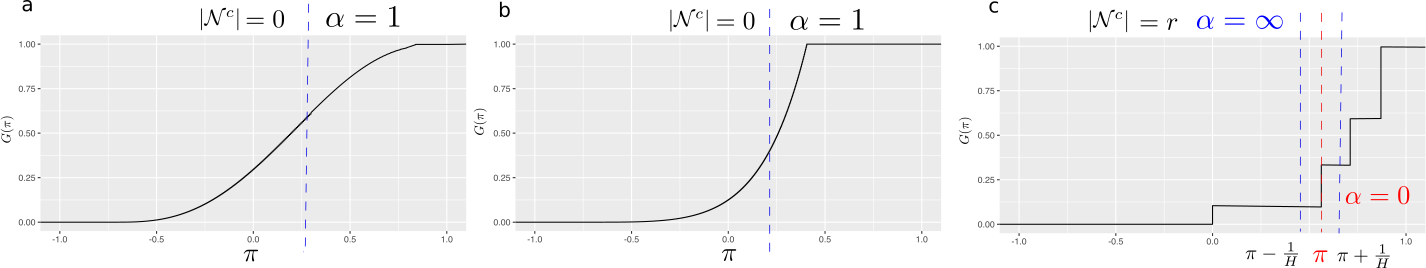
\includegraphics[width = \textwidth]{figure/cdf_new.pdf}
    \caption{Three examples of CDF with smoothness index $\alpha$ at $\pi$ depicted in dashed lines. Figure (a)-(b): Function $G(\pi)$ has $\alpha = 1$ with $\tN = \emptyset$, because the $G(\pi)$ has finite pseudo density in the range of $\pi$. Figure (c): Function $G(\pi)$ has $\alpha = \infty$ at most $\pi$'s (in blue), except for a total of $|\tN|_{\text{jump}}=r$ non-negligible jump points (in red).}
    \label{fig:cdf}
\end{figure}

\begin{rmk}[Interpretation of smoothness]
Figure~\ref{fig:cdf} illustrates three examples of the CDF with various $(\alpha,\tN)$. Here, the local $\alpha\geq 0$ quantifies the growth speed in $G$ at level $\pi$, and $|\tN|_{\text{jump}}\geq 0$ counts the non-negligible jump points, both accounting for a small tolerance $\Delta s$. The value of $\alpha$ depends on both the sampling distribution $\omega\sim \Pi$ and the behavior of $\Theta(\omega)$. A small value of $\alpha=0$ indicates heavy mass concentration at level $\pi$, or equivalently, when $G(\pi)$ jumps at $\pi$; a large value of $\alpha=\infty$ indicates nearly no concentration at level $\pi$, or equivalently, when $G(\pi)$ remains flat; an intermediate case is $\alpha = 1$ when $G(\pi)$ has a finite non-zero pseudo density in the vicinity of $\pi$.

%of $\alpha>1$, or equivalently, when $G(\pi)$ remains flat around $\pi$. A small value of $\alpha<1$ indicates the infinite density at level $\pi$, or equivalently, when the $G(\pi)$ jumps by greater than the tolerance $\Delta s$ at $\pi$. 

%Table~\ref{tab:simulation} illustrates the $G(\pi)$ for various models of $\Theta$ (see Section~\ref{sec:simulation}). 
\end{rmk}

We show that the $\alpha$-smoothness with $\alpha\neq 0$ implies the essential uniqueness for the risk minimizer in~\eqref{eq:optimal}. For two tensors $\Theta_1,\Theta_2$, define the mean absolute error (MAE) by
\[
\text{MAE}(\Theta_1, \Theta_2)=\mathbb{E}_{\omega\sim \Pi}|\Theta_1(\omega)-\Theta_2(\omega)|.
\]
We now reach the main theorem in this section. 

\begin{thm}[Perturbation bound of risk minimizer]\label{thm:population} Assume $\Theta\in\caliP(r)$ is $\alpha$-globally smooth. Then, for all $\pi\in \tN^c$ and all $\tZ\in\mathbb{R}^{d_1\times \cdots \times d_K}$, we have
\begin{align}\label{eq:identity}
&\textup{MAE}(\sign \tZ,\ \sign (\Theta-\pi)) \lesssim  C(\pi)\left[\textup{Risk}(\tZ)-\textup{Risk}(\Theta-\pi)\right]^{\alpha/(\alpha+1)} +\Delta s,
\end{align}
where $C(\pi)>0$ is a constant independent of $\tZ$; the specific form of $C(\pi)$ is provided in Appendix~\ref{sec:proofs}. In particular, when $\alpha\neq 0$, the risk minimizer is \emph{uniquely} equal to $(\Theta-\pi)$, up to sign equivalence and a small tolerance $\Delta s$. 
\end{thm}
%The bound~\eqref{eq:identity} immediately shows the uniqueness of the optimizer for $\text{Risk}(\cdot)$ up to a $\Delta s$-measure set under $\Pi$. We find that a higher value of $\alpha$ implies more stable recovery, as intuition would suggest. Similar results hold for optimization with sample risk~\eqref{eq:sample} (see Section~\ref{sec:estimation}). 


\begin{rmk}[Uniqueness and smoothness]
The bound~\eqref{eq:identity} bounds the deviation in $\text{MAE}(\cdot,\cdot)$ by the difference in $\textup{Risk}(\cdot)$. We conclude that the condition $\alpha\neq 0$ ensures the essential uniqueness of risk minimizer. Moreover, our result establishes the general recovery stability of sign tensor $\sign(\Theta-\pi)$ from weighted classification. The smoothness index $\alpha$ controls the worst-case perturbation around the risk minimizer $\sign(\Theta-\pi)$ with respect to the function $\textup{Risk}(\cdot)$. We find that a higher value of $\alpha$ implies more stable recovery.  This observation is consistent with intuition, because the best case $\alpha=\infty$ corresponds to easier estimation of $\sign(\Theta-\pi)$ with no point mass around decision boundary, whereas the worst case $\alpha = 0$ corresponds to hard estimation with a heavy mass around decision boundary. 

\end{rmk}
%The result establishes the recovery stability of sign tensors $\sign (\Theta-\pi)$ using optimization with population risk~\eqref{eq:population}. When $\alpha\neq 0$


\begin{rmk}[Comparison with hypergraphon models]\label{rmk:graphon}
Our notion of smoothness is related to, but also distinctive from, nonparametric hypergraphon models~\citep{xu2018rates,balasubramanian2021nonparametric}. In both approaches, the signal tensor is interpreted as a multivariate function from domain space $\mathbb{R}^{d_1\times \cdots \times d_K}$ to range space $[-1,1]$. Here, we consider an $\alpha$-smooth cumulative distribution function $G\colon[-1,1]\rightarrow\mathbb{R}$ in the range space; this is in contrast to nonparametric (hyper)graphon models that consider an $\alpha$-smooth multivariate function $f\colon \mathbb{R}^{d_1\times \cdots \times d_K}\rightarrow \mathbb{R}$ in the domain space. The localness in our approach is determined by the range space $[-1,1]$,  whereas the localness in (hyper)graphon model is determined by the domain space $[d_1]\times \cdots \times [d_K]$. The benefit bears the analogy of Lebesgue vs.\ Riemann integrals in functional analysis. The former is more appealing for tensor analysis, because the range space $[-1,1]$ is a simple scalar variable, whereas the domain space $[d_1]\times \cdots \times [d_K]$ is huge and multidimensional. 
\end{rmk}


\subsection{Why not $l_q$ weight for $q\neq 1$?}\label{sec:fail}
The weighted classification loss in \eqref{eq:sample} penalizes the sign mismatches by the magnitudes of deviation from level $\pi$. One may ask whether same conclusion holds by penalizing more (or less) on the magnitude of deviation. Specifically, we examine the generalized $l_q$ weighted classification risk defined by
\begin{align}\label{eq:gsample}
      \risk_q(\tZ) &= \mathbb{E}_{\omega\sim \Pi}\mathbb{E}_{\tY(\omega)}L_q(\tZ,\bar\tY_\Omega),\notag\\
 \text{where} \quad  L_q(\tZ,\bar\tY_\Omega) &= \frac{1}{|\Omega|}\sum_{\omega\in\Omega}|\bar\tY(\omega)|^q|\sign(\tZ(\omega))-\sign(\bar \tY(\omega))|.
 \end{align}
Here $q\geq 0$ is an integer controlling the penalization of magnitude $|\bar \tY(\omega)|$. We extend the our Theorem~\ref{prop:global} from $l_1$ weights to $l_q$ weights as follows.
\begin{thm}[Generalized weighted classification risk minimizer]\label{prop:global2}
Consider the same set-up as in Theorem~\ref{prop:global}. Then, we have\footnote{The expectation here is taken with respect to $\tY(\omega)$ for each $\omega$. For notational simplicity, the notion ``$=$'' in~\eqref{eq:optimal_detail} and~\eqref{eq:optimal_q} should be interpreted as ``one of the risk minimizers''(see Remark~\ref{rmk:landscape}). }
\begin{align}\label{eq:optimal_detail}
    \argmin_{ \tZ\in\mathbb{R}^{d_1\times \cdots \times d_K}}\textup{Risk}_q(\tZ) = 
    \begin{cases}\mathbb{E}(\tY-\pi)^q,& \text{if $q$ is an odd number},\\ \mathbb{E}\left[\tY-\pi\right]^q\mathds{1}\{\tY\geq \pi\}-\mathbb{E}\left[\tY-\pi\right]^q\mathds{1}\{\tY<\pi\},&\text{if $q$ 
     number.}
    \end{cases}
\end{align}
Furthermore, suppose either of the two conditions hold: (i) $p=1$, or (ii) $p\geq 0$ is a general integer, and the noise distribution $\tE(\omega)$ is symmetric around origin. Then, $(\Theta-\pi)$ minimizes the $l_q$ weighted classification risk; that is,
\begin{align}\label{eq:optimal_q}
  \argmin_{ \tZ\in\mathbb{R}^{d_1\times \cdots \times d_K}}\textup{Risk}_q(\tZ) = (\Theta-\pi).
\end{align}
\end{thm}

By convention, all expressions above should be interpreted in an entrywise fashion. Performance bounds similar to Theorem~\ref{thm:population} can be also derived for the generalized weighted classification risk minimizer. 
%Examination of the proof shows that, in the presence of non-symmetric error noise, we have 
%\begin{align}
   % \argmin_{ \tZ\in\mathbb{R}^{d_1\times \cdots \times d_K}}\textup{Risk}_q(\tZ) = \begin{cases}\sign(\mathbb{E}_{\tY(\omega)}\left(\tY-\pi)^q\right)& \text{ if $p$ is odd number},\\ \sign\left(\mathbb{E}_{\tY(\omega)\geq \pi}\left[\tY-\pi\right]^q-\mathbb{E}_{\tY(\omega)< \pi}\left[\tY-\pi\right]^q\right)&\text{ if $q$ is an even number.}
   % \end{cases}
%\end{align}
\begin{rmk}[Relationship between weights and noises]
Theorem~\ref{prop:global2} implies that, in the absence of symmetric noise, the generalized risk minimizer fails to recover $(\Theta-\pi)$ unless $p = 1$. For example, the risk minimizer becomes $(\text{Median}(\tE)+\Theta-\pi)$ when $p=0$ (i.e., the usual \emph{unweighted} classification risk). The solution fails when $\text{Median}(\tE)\neq 0$ in the absence of symmetry. The symmetric noise assumption is restrictive and often violated in practice. In particular, the distributions of Bernoulli, Binomial, Poisson residuals are intrinsically non-symmetric. Therefore, we choose $l_1$ weighted classification loss in~\eqref{eq:sample}. 
\end{rmk}


\section{Finite sample accuracy for signal tensor estimation}\label{sec:estimation}

In previous sections we have established the sign series representation and its relationship to weighted classification. In this section, we present the estimation of $\Theta \in \caliP(r)$ from sign tensor series. The main crux of our approach is a learning-reduction paradigm that connects a difficult $\mathbb{R}$-valued parameter estimation problem to a series of relatively simpler $\{0,1\}$-valued weighted classification problems. We develop the algorithm, provide the estimation error bound, and apply the results to various scenarios.


\subsection{Learning-reduction framework to signal estimation} 

Before describing our learning-reduction framework, we provide the intuition behind our method. In the two examples in Section~\ref{sec:motivation}, the high-rankness in the signal $\Theta$ makes the estimation challenging. Now let us examine the sign of the $\pi$-shifted signal $\sign(\Theta-\pi)$ for any given $\pi\in[-1,1]$. It turns out that, these sign tensors share the same sign patterns as low-rank tensors. Indeed, the signal tensor in Figure~\ref{fig:example}a-b has the same sign pattern as a rank-$4$ tensor, since $\sign(\Theta-\pi)=\sign(\tZ-f^{-1}(\pi))$. The signal tensor in Figure~\ref{fig:example}c has the same sign pattern as a rank-2 tensor, since $\sign(\Theta(i,j,k)-\pi)=\sign(\max(i,j,k)-d(e^{\pi}-1))$ (see Example~\ref{eq:example} in Section~\ref{sec:common}).

The above observation suggests a general framework to estimate sign-representable signal tensors. Figure~\ref{fig:demo} illustrates the main steps of our algorithm. We propose to estimate the signal tensor $\Theta\in\caliP(r)$ by taking the average over structured sign tensors
\begin{equation}\label{eq:est}
\hat \Theta = {1\over 2H+1}\sum_{\pi \in \tH}\sign{\hat \tZ_\pi}, \quad \text{with}\quad \hat \tZ_\pi = \argmin_{\tZ\colon \text{rank}\tZ\leq r} L(\tZ, \tY_\Omega-\pi),
\end{equation}
where $\tH=\{-1,\ldots,-{1/ H}, 0, {1/H},\ldots,1\}$ is the series of levels to consider, $H\in\mathbb{N}_{+}$ is a resolution parameter to be specified later (see Theorem~\ref{thm:estimation}), $L(\cdot,\cdot)$ is the $\ell_1$ weighted classification loss in~\eqref{eq:sample}, and the rank constraint on $\tZ$ follows from Theorem~\ref{prop:global}. 
%For the theory, we assume the true $r$ is known; in practice, $r$ could be chosen in a data adaptive fashion via cross-validation or elbow method~\citep{hastie2009elements}. 


%To obtain $\sign(\hat \tZ_\pi)$ for a given $\pi$, we dichotomize the data tensor into a sign tensor $\sign (\tY_\Omega-\pi)$ and estimate the de-noised sign by performing weighted classification. 

\begin{figure}[t]
\centerline{\includegraphics[width=\textwidth]{figure/demo.pdf}}
\caption{Illustration of our method in the context of an order-2 tensor (i.e. matrix). (a): a noisy, incomplete tensor input. (b)-(c): Estimation of sign tensor series $\sign(\Theta-\pi)$ for $\pi\in  \{-1,\ldots,-{1/ H},0,{1/H},\ldots,1\}$. (d): recovered signal $\hat \Theta$. The depicted signal is a full-rank matrix based on Example~\ref{eq:example} in Section~\ref{sec:common}.}\label{fig:demo}
\end{figure}

Our approach is built on the learning-reduction paradigm. We show that a careful aggregation of dichotomized data not only preserves all information in the original signals, but also brings benefits of accuracy and flexibility over classical low-rank models. Unlike traditional methods, the sign representation is guaranteed to recover both low- and high-rank signals. In addition, a \emph{polynomial} number of well-studied base problems suffice to recover $\Theta$ under the considered model (see the optimal choice of $H$ in Theorem~\ref{thm:estimation}). The method therefore enjoys both statistical effectiveness and computational efficiency. 

\subsection{Implementation details}
This section addresses the practical implementation of our estimation~\eqref{eq:est}. We take a divide-and-conquer approach by dividing the full procedure into a meta algorithm and $(2H+1)$ base algorithms. The meta algorithm takes the average of $(2H+1)$ sign tensors, whereas each base algorithm estimates the tensor $\sign(\Theta-\pi)$ given binary input $\sign(\tY_\Omega-\pi)$. The full procedure is described in Algorithm~\ref{alg:tensorT}.


\begin{algorithm}[h!]
  \caption{Nonparametric tensor completion via learning-reduction}\label{alg:tensorT}
 \begin{algorithmic}[1] 
\INPUT A noisy and possibly incomplete data tensor $\tY_\Omega$, rank $r$, resolution parameter $H$.
\For {$\pi \in \tH=\{ -1, \ldots, -{1\over H}, 0, {1\over H},\ldots, 1\}$}
%\State Define $\pi$-shifted tensor $\bar \tY=\tY-\pi$ and corresponding sign tensor $\sign(\bar \tY)=\sign(\tY-\pi)$. 
\State Base algorithm: Perform existing 1-bit tensor estimation algorithm~\citep{ghadermarzy2018learning,wang2018learning,hong2020generalized} on $(\tY_\Omega-\pi)$ and obtain 
\begin{align}\label{eq:base}
\hat \tZ_\pi=\argmin_{\tZ: \text{rank}(\tZ)\leq r} L(\tZ, \tY_\Omega-\pi).
\end{align}
\EndFor
\State Meta algorithm: Average over estimated sign tensors 
\begin{align}\label{eq:signal}
\hat \Theta={1\over 2H+1}\sum_{\pi \in \tH}\sign(\hat \tZ_\pi).
\end{align}
\OUTPUT Estimated signal tensor $\hat \Theta$.
\end{algorithmic}
\end{algorithm}

The base algorithm~\eqref{eq:base} reduces to a well-studied low-rank 1-bit tensor estimation problem. A number of efficient algorithms with convergence guarantees are readily available for this problem~\citep{ghadermarzy2018learning,wang2018learning,hong2020generalized,han2020optimal}. For example, \cite{wang2018learning} developed an alternating optimization algorithm, and \cite{han2020optimal} developed a projected gradient descent algorithm. For self-containedness, we summarize the alternating optimization algorithm here. More details can be found in previous work~\citep{wang2018learning,hong2020generalized}. Briefly, we use the rank decomposition~\eqref{eq:CP} of $\tZ=\tZ(\mA_1,\ldots,\mA_K)$ to optimize the unknown factor matrices $\mA_k=[\ma^{(k)}_1,\ldots,\ma_r^{k}]\in\mathbb{R}^{d_k\times k}$, where tensor singular values are collected into the last factor $\mA_K$. We numerically solve~\eqref{eq:base} by optimizing one factor $\mA_k$ at a time while holding others fixed. Each suboptimization reduces to a simple classification problem with classical vector-based decision variable. Following common practice in tensor optimization, we run the optimization from multiple initializations to locate a final estimate with the lowest objective value. 

We emphasize that we did not attempt to propose a new base algorithm for~\eqref{eq:base} and its algorithmic convergence; indeed, both are not new in the literature. Our major contribution is a learning-reduction framework by adopting existing algorithms for a more challenging high-rank problems. We will show this approach achieves statistical-computational efficiency almost for free, i.e., at almost no extra statistical cost and only an extra $\text{poly}(d)$ computational cost (see Theorem~\ref{thm:estimation}). The developed sign-representable tensor model unifies low-rank and high-rank tensors, thereby empowering exiting algorithms for broader implications.

In theory, extra technical assumptions are needed for the algorithmic convergence of the base algorithm~\citep{wang2018learning,han2020optimal}. We omit the details here but instead assume the estimate~\eqref{eq:base} is attainable. We also note the existence of several 1-bit tensor algorithms that use surrogate loss~\citep{genzel2020robust,he2017kernelized} instead of the loss in~\eqref{eq:est}. Under certain regularity conditions, these algorithms can also be adopted in our setting. More details on the implementation will be discussed in Section~\ref{sec:implementation}. 

\begin{rmk}[Distinction between our algorithm and classical 1-bit tensor algorithm] 
The key novelty in our algorithm compared to classical 1-bit tensor algorithm lies in the aggregation step~\eqref{eq:signal}. Classical tensor algorithm takes $\hat \tZ_\pi$ as output. By contrast, we dichotomize the estimate $\hat \tZ_\pi$ by ignoring its magnitude, and then aggregate the sign series $\sign(\hat \tZ_\pi)$ into a new continuous-valued estimator $\hat \Theta$. Somewhat surprisingly, we find that the dichotomization not only preserves all information in the original signals, but also brings benefits of accuracy and flexibility over classical parametric methods. 
\end{rmk}

%For the theory, we assume the true $r$ is known; in practice, $r$ could be chosen in a data adaptive fashion via cross-validation or elbow method~\citep{hastie2009elements}. Furthermore, we assume the technical assumptions for the base algorithm are satisfied such that~\eqref{eq:base} is attainable. More details on the implementation will be discussed in Section~\ref{sec:implementation}. 


\subsection{Finite sample accuracy}\label{sec:error}
%For a cleaner exposition, we assume the noise is bounded and the range of $Y$ is in $[-1,1]$; the extension  to various types of noise is provided in Section~\ref{sec:subGaussian}. 

Given a noisy incomplete tensor observation $\tY_\Omega$ from model~\eqref{eq:model}, we cast the problem of estimating $\Theta\in\caliP(r)$ into a series of weighted classifications. We are particularly interested in the high-dimensional region, where $\min_{k\in[K]}{d_k} \to \infty$ while holding $r\lesssim \tO(1)$ as fixed. For a cleaner exposition, we assume the loss~\eqref{eq:sample} is bounded by a universal constant; the extension to unbounded loss is provided in Section~\ref{sec:extension}. The next theorem establishes the finite sample accuracy for the estimates from Algorithm~\ref{alg:tensorT}. 

\begin{thm}[Estimation error for sign representable tensors]\label{thm:estimation} Consider the model~\eqref{eq:model} with $\Theta\in\caliP(r)$. Suppose $\Theta(\omega)$ is an $\alpha$-globally smooth tensor with non-negligible jump points collected in set $\tN$. Let $\hat \tZ_\pi$ and $\hat \Theta$ denote the estimates in~\eqref{eq:base} and~\eqref{eq:signal} from Algorithm~\ref{alg:tensorT}, respectively. Denote 
\[ 
d_{\max}=\max_{k\in[K]}d_k,\quad \text{and}\quad t_d = {d_{\max}r\log|\Omega|\over |\Omega|}.
\]
Under the bounded loss assumption, we have the following error bounds with a high probability at least $1-\exp(-d_{\max}t_d)$.
\begin{enumerate}[label=(\alph*)]
\item (Sign tensor estimation). For all $\pi\in\tN^c$,
\begin{equation}\label{eq:bound}
\textup{MAE}(\sign(\hat \tZ_\pi),\ \sign(\Theta-\pi)) \lesssim t_d^{\alpha\over \alpha+2}+{1\over \rho^2(\pi,\tN)}t_d.
\end{equation}
\item (Signal tensor estimation). For any resolution parameter $H\in\mathbb{N}_{+}$,
\begin{equation}\label{eq:bound2}
\textup{MAE}(\hat \Theta,\ \Theta)\lesssim \KeepStyleUnderBrace{(t_d\log H)^{\alpha\over \alpha+2}}_{\text{error inherited from sign estimation}}+\KeepStyleUnderBrace{{1+|\tN|_{\text{jump}}\over H}}_{\text{bias}}+\ \KeepStyleUnderBrace{{t_d(H\log H)}}_{\text{variance}}.
\end{equation}
In particular, setting $\scriptstyle  H=\sqrt{(1+|\tN|_{\text{jump}})/t_d}\ \lesssim \text{ poly}(d_{\max})$ yields the tightest upper bound in~\eqref{eq:bound2}.
\end{enumerate}
\end{thm}


%\begin{thm}[Sign tensor estimation error]\label{thm:classification} Suppose $\Theta\in\caliP(r)$ and $\Theta(\omega)$ is $\alpha$-globally smooth under $\omega\sim \Pi$. Let $\hat \tZ_\pi$ be the estimate in~\eqref{eq:est} and $d=\max_{k\in[K]}d_k$. Then, for all $\pi\in\tN^c$, with very high probability over $\tY_\Omega$, 
%\begin{equation}\label{eq:bound2}
%\textup{MAE}(\hat \Theta,\ \Theta)\lesssim \KeepStyleUnderBrace{(t_d\log H)^{\alpha\over \alpha+2}}_{\text{error inherited from sign estimation}}+\KeepStyleUnderBrace{{1+|\tN|\over H}}_{\text{bias}}}+\ \KeepStyleUnderBrace{{t_dH\log H}}_{\text{variance}}.
%\end{equation}
%\end{thm}

In the special case of full observation with equal dimension $d_1=\cdots=d_K=d$ and bounded $|\tN|_{\text{jump}}\lesssim \tO(1)$, our signal tensor estimate achieves convergence
\begin{equation}\label{eq:special}
\textup{MAE}(\hat \Theta, \Theta)\lesssim rd^{-(K-1)\min({\alpha\over \alpha+2},\ {1\over 2})}\log^2 d, \quad \text{by setting}\ H\asymp d^{(K-1)/2}.
\end{equation}
Compared to earlier methods, our estimation accuracy applies to both low- and high-rank signal tensors. The rate depends on the sign complexity $\Theta\in\caliP(r)$, and this $r$ is often much smaller than the usual tensor rank (see Proposition~\ref{cor:monotonic}). Our result also reveals that the convergence becomes favorable as the order of data tensor increases. 



\begin{rmk}[Sign estimation compared to existing work]
The bound~\eqref{eq:bound} is a finite-sample version of Theorem~\ref{thm:population}. The result demonstrates the polynomial decay of sign errors with sample size $|\Omega|$. 
%The result demonstrates the polynomial decay of sign errors with $|\Omega|$. Our sign estimate achieves consistent recovery using as few as $\tilde \tO(dr)$ noisy entries. 
Our error bound~\eqref{eq:bound} improves the existing work on weighted classification. Existing work~\citep{tsybakov2004optimal,xu2020class} considered only a finite number of $\pi$'s, and provided only the first term in the bound~\eqref{eq:bound}. By contrast, our bound quantifies the full dependence on the level $\pi$ and establishes the recovery of $\sign(\Theta-\pi)$ \emph{uniformly} over all possible $\pi\in\tN^c$. It turns out both terms in the bound~\eqref{eq:bound} are crucially in the signal error bound in~\eqref{eq:bound2}: the first term contributes to the inherited sign estimation error, whereas the second term contributes to the variance term in sign averaging. 
\end{rmk}

%Recall that $|\tN|_{\text{jump}}$ counts the non-negligible jump points in the distribution~\eqref{eq:cdf}. Combining the sign representability of the signal tensor and the sign estimation accuracy, we obtain our main results on nonparametric tensor estimation. 

%\begin{thm}[Signal tensor estimation error]\label{thm:estimation} Consider the same conditions of Theorem~\ref{thm:classification}. Let $\hat \Theta$ be the estimate in~\eqref{eq:est}. For any resolution parameter $H\in\mathbb{N}_{+}$, with very high probability over $\tY_\Omega$,
%\begin{equation}\label{eq:bound2}
%\textup{MAE}(\hat \Theta,\ \Theta)\lesssim \KeepStyleUnderBrace{(t_d\log H)^{\alpha\over \alpha+2}}_{\text{error inherited from sign estimation}}+\KeepStyleUnderBrace{{1+|\tN|\over H}}_{\text{bias}}}+\ \KeepStyleUnderBrace{{t_dH\log H}}_{\text{variance}}.
%\end{equation}
%In addition, setting $\footnotesize H= (1+|\tN|)^{1/2} t_d^{-1/2}\asymp \text{poly}(d)$ yields the tightest upper bound in~\eqref{eq:bound2}.
%\end{thm}



\begin{rmk}[Signal estimation]
The bound~\eqref{eq:bound2} demonstrates our main results for nonparametric signal estimation. We make three remarks. 

$\bullet$ (Error decomposition) The bound~\eqref{eq:bound2} reveals three sources of errors: the estimation error for sign tensors, the bias from sign series representations, and the variance thereof. The resolution parameter $H\in\mathbb{N}_{+}$ determine the number of sign tensors to average in the estimation. The best choice of $H=\sqrt{(1+|\tN|_{\text{jump}})/t_d}$ balances the bias-variance tradeoff. A larger value of $H$ reduces the approximation bias but renders the sign estimation harder near mass points, and vice versa. 

$\bullet$ (From sign to signal estimation) We find that the signal estimation error~\eqref{eq:bound2} is generally no better than the corresponding sign error~\eqref{eq:bound}. In the special case as in~\eqref{eq:special} with $\alpha=\infty$, the sign estimation~\eqref{eq:bound} reaches a fast rate $\tO(d^{-(K-1)})$ whereas the signal tensor estimation reaches a slow rate $\tO(d^{-(K-1)/2})$. 
The phenomenon is to be expected, since magnitude estimation is harder than sign estimation. 

$\bullet$ (Robustness) We also find that the signal estimation is robust to finitely many off-target sign estimations, as long as the majorities are accurate. This can be seen by the order equivalence of $|\tN|_{\text{jump}}=0$ vs.\ $|\tN|_{\text{jump}}\asymp \tO(1)$ in the bound~\eqref{eq:bound2}. Recall that $|\tN|_{\text{jump}}$ counts the non-negligible jump points for which sign tensors are nonrecoverable from classification risks (see red line in Figure~\ref{fig:cdf}c). Nevertheless, the signal tensor is still estimable, because the nearby sign estimations (blue lines in Figure~\ref{fig:cdf}c) provide the magnitude information. The fact shows the benefit of sign aggregation approach to signal estimation. 
\end{rmk}

\begin{rmk}[Technical novelty in the proof] The main challenge in the proof of Theorem~\ref{thm:estimation} is that our estimates are \emph{not} likelihood-based. In particular, our loss function is not restricted to a particular noise distribution; instead only weak first-order moment assumption is invoked. Such flexibility renders classical likelihood-based tensor analysis~\citep{wang2018learning, ghadermarzy2018learning,zhang2018tensor} non-applicable in our setting. We develop new empirical process tools to address this challenge. 

The proof of Theorem~\ref{thm:estimation} consists of three main ingredients. We first leverage the $\alpha$-smoothness to provide a sharp classification error faster than the usual root-$n$ convergence. The improvement stems from a variance-to-mean relationship in classification loss and a careful \emph{local} analysis of empirical process (see Appendix~\ref{sec:novalty}). The result implies that, in the local region of risk minimizer $\sign(\Theta-\pi)$, the estimate $\hat \tZ_\pi$ converges more quickly than the simple uniform convergence results would suggest. The second step is to convert the risk error into the mean absolute error by Theorem~\ref{thm:population}. The last step is to aggregate the sign errors into the continuous-valued signal estimation error. A careful error analysis reveals the joint contribution from both sign aggregations and variance-bias trade-off.
\end{rmk}



Finally, we apply our Theorem~\ref{thm:estimation} to the problem of tensor completion. The following corollary reveals the sample complexity for nonparamtric tensor completion. 
\begin{cor}[Sample complexity for nonparametric completion]\label{cor:completion}Assume the same conditions of Theorem~\ref{thm:estimation} and bounded $|\tN|_{\text{jump}}$. Then, with a high probability at least $1-\exp(-d_{\max}t_d)$,
\[
\textup{MAE}(\hat \Theta, \Theta)\to 0, \quad \text{as}\quad {|\Omega|\over {d_{\max}r} \log^2 |\Omega|}\to \infty.
\]
\end{cor}
Our result improves earlier work~\citep{yuan2016tensor,ghadermarzy2019near,pmlr-v119-lee20i} by allowing both low- and high-rank signals. Interestingly, the sample requirements depend only on the sign complexity $(d_{\max}r)$ but not the nonparametric complexity $\alpha$. Note that $\tilde \tO(d_{\max}r)$ roughly matches the degree of freedom of sign tensors, suggesting the optimality of our sample requirements. 


\subsection{Revisiting earlier examples}
We apply our method to the main examples in Section~\ref{sec:common}. For simplicity, suppose $\omega\sim \Pi$ is the uniform sampling. The comparison with existing literature is summarized in Table~\ref{tb:comparison}. Numerical comparisons are provided in Section~\ref{sec:simulation}. 

\begin{customexample}{2}[TBMs]
Consider a tensor block model with $r$ multiway blocks. The tensor block model $\Theta\in \caliP(r)$ is $\infty$-globally smooth. The number of non-negligible jump points $|\tN|_{\text{jump}}$ equals the number of distinct values in $\Theta$. The CDF $G$ satisfies $\alpha= \infty$ for all regular $\pi$'s, since no point mass at $\pi\in \tN^c$ (see Figure~\ref{fig:cdf}c for an example). Applying our Theorem~\ref{thm:estimation} implies a rate $\tilde \tO(d^{-(K-1)/2})$ by taking $\alpha=\infty$ and $|\tN|_{\text{jump}} \leq r\lesssim \tO(1)$. This rate agrees with the  previous root-mean-square error (RMSE) for block tensor estimation~\citep{wang2019multiway}. The rate is known to be minmax optimal, thereby suggesting the sharpness of our bound in this example. 
\end{customexample}

\begin{customexample}{3} [GLMs] 
Consider a GLM tensor $\Theta=g(\tZ)$, where $g$ is a known link function and $\tZ$ is a latent low-rank tensor. Suppose the CDF of $\Theta$ has bounded pseudo density with $\alpha=1$ (see Figure~\ref{fig:cdf}b-c for an example). Applying our Theorem~\ref{thm:estimation} yields the estimation error $\tilde \tO(d^{-(K-1)/3})$. This rate is slightly slower than the parametric RMSE rate~\citep{zhang2018tensor,wang2018learning}, as expected. The reason is that our estimate remains valid for unknown $g$ and high-rank tensors. The nonparametric rate is the price one has to pay for not knowing the form $g(\cdot)$ as a priori. 
\end{customexample}

\begin{customexample}{4}[SIMs]
The earlier example has shown the nonparametric rate $\tilde \tO(d^{-(K-1)/3})$ when applying our method to single index tensor model. In the matrix case with $K=2$, our result yields error rate $\tilde \tO(d^{-1/3})$, which is faster than the RMSE rate $\tO(d^{-1/4})$ obtained by \cite{ganti2015matrix}. Recent work~\citep{xu2018rates} establishes the RMSE rate $\tilde \tO(d^{-1/3})$ for Lipschitz bivariate graphon models for matrices.  The rate is a special case of our Theorem~\ref{thm:estimation} by setting tensor order $K=2$, thereby suggesting the sharpness of our error bound. 
\end{customexample}

\begin{customexample}{5}[Structured tensors with repeating entries]

Consider the high-rank order-$K$ $(d,d,d)$-dimensional tensor with entries $\Theta(i_1,\cdots,i_K) = \log(1+\max_{k\in[K]}i_k/d)$. We have known $\Theta\in \caliP(r)$ from Section~\ref{sec:common}. Now we conclude $\Theta$ is $\infty$-globally smooth. The number of non-negligible jump points equals $d$, because $|\tN|_{\text{jump}}= \text{Card}\{\log(1+i/d):i\in[d]\}=d$, where $\text{Card}\{\cdot\}$ denotes the cardinality of the set. The CDF $G$ satisfies $\alpha= \infty$ for all $\pi\in \tN^c$. Applying our Theorem~\ref{thm:estimation} with $\alpha=\infty$ and $|\tN|_{\text{jump}}=d$ yields the rate $\tilde \tO(d^{-(K-2)/2})$. 
\end{customexample}

\begin{table}
\resizebox{\textwidth}{!}{
\begin{tabular}{l|l|l|l|l}
\multicolumn{1}{c|}{Model}   & $\alpha$    & $|\tN|_{\text{jump}}$  & Our rate (power of $d$) & \multicolumn{1}{c}{Comparison with previous results} \\\hline
\multirow{2}{*}{Sign representable tensor}                                   & \multirow{2}{*}{$\geq 0$}    &   \multirow{2}{*}{Finite}    &   \multirow{2}{*}{$-(K-2)\min(\frac{\alpha}{\alpha+2},\frac{1}{2})$} & \multirow{2}{*}{New.} \\
&&&&\\
\hline
\multirow{2}{*}{Tensor block model } & \multirow{2}{*}{$\infty$} & \multirow{2}{*}{Finite} &          \multirow{2}{*}{$-(K-1)/2$}            & \multirow{2}{*}{Minimax optimal as in \citep{wang2019multiway}}\\
&&&&\\
\multirow{2}{*}{Single index model} &\multirow{2}{*}{1}       & \multirow{2}{*}{0}  &  \multirow{2}{*}{$-(K-1)/3$ }                    & New for general $K>3$;   Improves   the previous         \\
&&&& rate -1/4 for $K=2$ \citep{ganti2015matrix}.  \\
\multirow{2}{*}{Generalized linear model }                &\multirow{2}{*}{1}        &\multirow{2}{*}{0}  &       \multirow{2}{*}{$-(K-1)/3$}  &  \multirow{2}{*}{Close to minimax rate~\citep{wang2018learning}.}   \\
&&&&\\
\multirow{2}{*}{Structure with repeating entries}   & \multirow{2}{*}{$\infty$}   & \multirow{2}{*}{$d$}       &      \multirow{2}{*}{$-(K-2)/2$ }   & \multirow{2}{*}{New.}                       \\
&&&&\\
\end{tabular}
}
\caption{Summary of our statistical rates compared to existing works under different models.  For notational simplicity, we present error rates assuming equal tensor dimension in all modes and finite $|\tN|_{\text{jump}}$ for the smooth tensor model. Here $K\geq 2$ denotes the tensor order and $d$ denotes the tensor dimension.}
\label{tb:comparison}
\end{table}


\section{Extensions}\label{sec:extension}


Recall our signal plus noise model in \eqref{eq:model},
\begin{align*}
\tY = \Theta+\tE,\quad \mathbb{E}(\tE)=0,
\end{align*}
where $\Theta\in\caliP(r)$ is an $\alpha$-smooth sign representable signal tensor of interest, and $\tE$ consists of zero-mean, independent noise entries. In our main theory of earlier sections~\ref{sec:stat}-\ref{sec:estimation}, we have imposed rather weak assumptions on the noise, in that only three aspects are invoked: (i) entrywise independence of $\tE$ (conditional on $\Theta$), (ii) zero-mean constraint $\mathbb{E}(\tE) = 0$; and (iii) boundedness of weighted loss (for finite sample accuracy results only). Other aspects of the noise (e.g.\ variance, symmetry, distribution) are irrelevant. In this section, we specialize our results to various problems and provide extension to unbounded weighted loss. 

\subsection{Sub-Gaussian tensor denoising} Sub-Gaussian tensor denoising is a popular problem in literature. A range of parametric structures have been considered in earlier work, including CP-low rankness~\citep{anandkumar2014tensor}, sparsity~\citep{allen2012sparse}, and blockness~\citep{wang2019multiway}. Here, we generalize our nonparametric sign representable model~\eqref{eq:model} to sub-Gaussian tensor denoising problem.  
Specifically, suppose the noise tensor $\tE$ in~\eqref{eq:model} consists of zero-mean, independent sub-Gaussian entries with variance bounded by $\sigma^2$. 
\begin{assumption}[Sub-Gaussian noise]\label{assm:subg}
%\item There exists a constant $\beta>0$, independent of tensor dimension, such that $\|\Theta\|_\infty\leq \beta$. Without loss of generality, we set $\beta = 1$.
The noise entries $\tE(\omega)$ are independent zero-mean sub-Gaussian random variables with variance proxy $\sigma^2>0$; i.e, 
\[
\mathbb{P}(|\tE(\omega)|\geq B)\leq 2e^{-B^2/2\sigma^2},\  \text{for all}\ B>0.
\] 
%\end{enumerate}
\end{assumption}
The sub-Gaussian noise satisfies the aforementioned noise assumptions (i)-(ii) but not (iii). In particular, the classification loss~\eqref{eq:sample} becomes unbounded due to the presence of weights $|\bar \tY(\omega)|$. The following Corollary provides our nonparametric estimation error for sub-Gaussian tensor denoising. 

\begin{cor}[sub-Gaussian tensor denoising with nonparametric signals]\label{thm:unbddno1}
Consider the same setup as in Theorem~\ref{thm:estimation}. Suppose that Assumption~\ref{assm:subg} is used in place of the bounded loss assumption. For simplicity, assume $|\tN|_{\text{jump}}\lesssim \tO(1)$ and $d_1=\cdots =d_K=d$. Set
\[
t_d ={ \sigma^2d r\log d \log |\Omega|\over |\Omega|} \quad \text{and}\quad H\asymp \sqrt{1\over t_d}.
\] 
Then, with a high probability at least $1-\exp(-d t_d)$,
\begin{equation}\label{eq:bound3}
%\textup{MAE}(\hat \Theta, \Theta)\lesssim \left(t_d\log H\right)^{\alpha \over \alpha+2}+{1+|\tN|_{\text{jump}}\over H}+{H( t_d\log H)},\text{ where } t_d :={ r\sigma^2d_{\max}\log d_{\max}\log |\Omega|\over |\Omega|}.\\
\textup{MAE}(\hat \Theta, \Theta)\lesssim t_d^{\min\left({\alpha\over \alpha+2}, {1\over 2}\right)}.
\end{equation}
%In particular, setting $H\asymp \sqrt{(1+|\tN|_{\text{jump}})/ t_d}$ yields the tightest upper bound in~\eqref{eq:bound3}.
\end{cor}
We find that the (unbounded) sub-Gaussian noise incurs only an additional $\log d$ factor compared to Theorem~\ref{thm:estimation}. 



\subsection{Probabilistic tensor estimation}
Binary tensor problems commonly arise in recommendation system and network analysis. Examples include context-based recommendation system~\citep{adomavicius2011context}, multi-relational social networks~\citep{nickel2011three}, and brain connectivity network~\citep{wang2019common}. Here, we generalize our nonparametric model to binary tensors.

Specifically, assume that we observe a binary tensor $\tY\in\{0,1\}^{d_1\times \cdots\times d_K}$  
whose entries are realizations of independent Bernoulli random variables, such that,
\begin{align}\label{eq:bernoulli}
    \tY(\omega)\sim \text{Bernoulli}\left(\Theta(\omega)\right), \ \text{for all}\ \omega\in \Omega. 
\end{align}
Here the signal tensor, $\Theta\in\caliP(r)$, represents the probability tensor of interest. Notice that model~\eqref{eq:bernoulli} can be represented as the additive model~\eqref{eq:model}, by setting the noise as the Bernoulli residual $\tE=\tY-\Theta$. Since the weighted loss~\eqref{eq:sample} is bounded in this setting, directly applying Theorems~\ref{thm:estimation} yields the estimation error.

\begin{cor}[Probabilistic tensor estimation with nonparametric signals]\label{thm:bernoulli}
Consider the same setup as in Theorem~\ref{thm:estimation}. Suppose a binary tensor is observed from \eqref{eq:bernoulli}. 
%Then, for any resolution parameter $H\in\mathbb{N}_{+}$, with a high probability at least $1-\exp(-d_{\max}t_d)$,
For simplicity, assume $|\tN|_{\text{jump}}\lesssim \tO(1)$ and $d_1=\cdots =d_K=d$. Set
\[
t_d ={d r \log |\Omega|\over |\Omega|} \quad \text{and}\quad H\asymp \sqrt{1\over t_d}.
\] 
Then, with a high probability at least $1-\exp(-d t_d)$,
\begin{equation}\label{eq:bound4}
\textup{MAE}(\hat \Theta, \Theta)\lesssim t_d^{\min\left({\alpha\over \alpha+2}, {1\over 2}\right)}.
%\textup{MAE}(\hat \Theta, \Theta)\lesssim \left(t_d\log H\right)^{\alpha\over \alpha+2}+{1+|\tN|_{\text{jump}}\over H}+{H( t_d\log H)},\text{ where } t_d :={ d_{\max}r\log |\Omega|\over |\Omega|}.
\end{equation}
%In particular, setting $H\asymp \sqrt{(1+|\tN|_{\text{jump}})/ t_d}$ yields the tightest upper bound in~\eqref{eq:bound4}.
\end{cor}
We find that the entries of nonparametric tensor estimator $\hat \Theta$ automatically fall into the valid probability range $[0,1]$. This is because in the aggregation step~\eqref{eq:signal}, the sign tensors $\sign(\hat \tZ_\pi)=\mathbf{1}\otimes \cdots \otimes \mathbf{1}$ are constant tensors for a total of $(H+1)$ non-positive levels $\pi\leq 0$. Therefore, $\hat \Theta(\omega) \in [{(H+1)-H\over 2H+1}, {(H+1)+H\over 2H+1}]\subset [0,1]$.

\subsection{Binomial tensor problem} 

Binomial tensor problems appear when the observations are success counts from a limited numbers of trails. For example, the human mortality databset~\citep{jdanov2019human} provides the death counts and the total numbers of individuals for each combination (country, age, year). This dataset is naturally summarized as a three-way tensor of $\text{country}\times\text{age}\times\text{year}$, where the entries can be modeled as independent binomial trials. Here, we generalize our nonparametric model to binomial tensors.

Specifically, suppose that we observe a success count tensor $\tY\in\mathbb{N}^{d_1\times\cdots\times d_K}$ from a total trial count tensor $\tP\in\mathbb{N}_{+}^{d_1\times \cdots\times d_K}$, where $0\leq \tY\leq \tP$ in an entrywise fashion. Assume that $\tY$ consists of independent binomial counts given the total trial counts $\tP$, such that,
\begin{align}
\label{eq:binom}
    \tY(\omega) \sim \text{Binomial}\left(\tP(\omega),\Theta(\omega)\right), \quad \text{for all } \omega\in\Omega. 
\end{align}
The goal is to estimate the success probability $\Theta\in\caliP(r)$ from the observed tensor $\tY_\Omega$ given total trial counts $\tP$. Then, we have the following theoretical guarantee for the binomial tensor model.

\begin{cor}[Binomial tensor problem with nonparametric signals]\label{thm:binom}
Consider the same setup as in Theorem~\ref{thm:estimation}. Suppose a success count tensor is observed from \eqref{eq:binom}. For simplicity, assume $|\tN|_{\text{jump}}\lesssim \tO(1)$, $\maxnorm{\tP}\lesssim \tO(1)$, and $d_1=\cdots=d_K=d$. Set
\[
t_d ={d r \log |\Omega|\over |\Omega|} \quad \text{and}\quad H\asymp \sqrt{1\over t_d}.
\] 
%Then, for any resolution parameter $H\in\mathbb{N}_{+}$, with a high probability at least $1-\exp(-d_{\max}t_d)$,
Then, with a high probability at least $1-\exp(-d t_d)$,
\begin{equation}\label{eq:bound5}
%\textup{MAE}(\hat \Theta, \Theta)\lesssim \frac{1}{p}\left[\left(t_d\log H\right)^{\alpha \over \alpha+2}+{1+|\tN|_{\text{jump}}\over H}+{H( t_d\log H)}\right],\text{ where } t_d ={ d_{\max}r\log |\Omega|\over |\Omega|}.
\textup{MAE}(\hat \Theta, \Theta)\lesssim \frac{1}{\min_{\omega\in[d_1]\times\cdots\times[d_K]}\tP(\omega)}{t_d^{\min\left({\alpha\over \alpha+2}, {1\over 2}\right)}}.
\end{equation}
%In particular, setting $H\asymp \sqrt{(1+|\tN|_{\text{jump}})/ t_d}$ yields the tightest upper bound in~\eqref{eq:bound5}.
\end{cor}
Corollary~\ref{thm:binom} is a generalization of Corollary~\ref{thm:bernoulli} from Bernoulli trails with $\tP=\mathbf{1}\otimes \cdots \otimes \mathbf{1}$ to Binomial trials with general $\tP\in\mathbb{N}_{+}^{d_1\times \cdots \times d_K}$. 

\subsection{Extension to hinge loss}\label{sec:implementation}
In earlier sections, we have established our main results under the weighted classification loss 
\begin{equation}
L(\tZ, \bar \tY_\Omega)= {1\over |\Omega|}\sum_{\omega \in \Omega}\ \KeepStyleUnderBrace{|\bar \tY(\omega)|}_{\text{$l_1$ weight}}\  \times \ \KeepStyleUnderBrace{| \sign \tZ(\omega)-\sign \bar \tY(\omega)|}_{\text{classification loss}},
\end{equation}
where $|\sign(\tZ)-\sign(\bar \tY)|$ is the canonical classification loss. Here, we generalize the canonical classification loss $\ell(z,y)=|\sign z - \sign y|$ to (unbounded) hinge loss $F(m) = (1-m)_+$. 
Hinge loss is commonly used as a surrogate classification loss due to its continuity~\citep{bartlett2006convexity,genzel2020robust,he2017kernelized}. 

Specifically, we establish the parallel theory of Theorem~\ref{thm:estimation} for hinge loss. The only difference in setup is that, the estimates $\tZ_\pi$, $\hat \Theta$ in~\eqref{eq:base}-\eqref{eq:signal} are now replaced by
\begin{align}\label{eq:hingeest}
\hat \tZ_{\pi,F}= \argmin_{\rank(\tZ)\leq r}\sum_{\omega\in \Omega} |\bar \tY(\omega)|F(\tZ(\omega)\sign\bar \tY(\omega))+\lambda_\pi \FnormSize{}{\tZ}^2,\quad \hat \Theta_F={1\over 2H+1}\sum_{\pi \in \tH}\sign(\hat \tZ_{\pi,F}),
\end{align} 
where $F(\cdot)=(1-m)_{+}$ is the hinge loss, and $\lambda_\pi>0$ is the penalty parameter. We use $\risk_F(\cdot)$ to denote the \emph{surrogate weighted classification loss}, defined similarly as in~\eqref{eq:population}, with hinge loss used in place of canonical loss. A nice property of hinge loss is the following \emph{Fisher consistency bound}~\citep{scott2011surrogate},
%Notice that the choice of hinge loss implies the Fisher consistency bound for the weighted risk \citep{scott2011surrogate},
\begin{equation} \label{eq:fisher}
\risk(\tZ)-\risk(\Theta-\pi)\lesssim \risk_{F}(\tZ)-\risk_{F}(\Theta-\pi), \text{ for all $\pi\in[-1,1]$ and all tensors $\tZ$}.
\end{equation}
The Fisher consistency enables us to relate the excess risk of the hinge loss to that of canonical loss.

\begin{assumption}[Approximation bias]\label{ass:loss} 
Denote $n=|\Omega|$. For all $\pi\in\tN^c$, assume there exist a sequence of tensors $\tZ^{(n)}_\pi\in\caliP(r)
$, such that $\risk_F(\tZ^{(n)}_\pi)-\risk_F(\Theta-\pi)\leq a_n$, for some sequence $a_n\to 0$ as $n\to\infty$. Furthermore, assume $\FnormSize{}{\tZ_{\pi}^{(n)}} \leq J$ for some constant $J>0$. 
\end{assumption}


Assumption~\ref{ass:loss} quantifies the representation capability of $\caliP(r)$ for the true $\text{sign}(\Theta-\pi)$.  Under Assumption \ref{ass:loss}, the hinge estimate~\eqref{eq:hingeest} enjoys statistical efficiency. 
\begin{thm}[Hinge loss based estimation]~\label{thm:extension} 
Consider the same setup as in Theorem~\ref{thm:estimation}. For simplicity, assume $|\tN|_{\text{jump}}\lesssim \tO(1)$ and $d_1=\cdots=d_K=d$. Denote
\[
n=|\Omega|, \quad t_n={ r d \log n \over n}, \quad \lambda_\pi\asymp t_n^{\alpha+1\over \alpha+2}+{t_n\over\rho(\pi,\tN)}, \ \text{and}\ H\asymp \sqrt{1\over t_n}.
\]
Suppose the Assumption~\ref{ass:loss} with $a_n \lesssim t_n^{(\alpha+1)/(\alpha+2)}$ holds in place of the bounded loss assumption. Then, with a high probability at least $1-\exp(-nt_n)$,
%\begin{enumerate}[label=(\alph*)]
%\item (Sign tensor estimation). For all $\pi\in[-1,1]$ except for a finite number of levels,
%\begin{equation}\label{eq:sfe}
%\textup{MAE}(\sign(\hat \tZ_\pi),\ \sign(\Theta-\pi)) \lesssim t_n ^{\alpha\over 2+\alpha}+{1\over \rho^2(\pi,\tN)}t_n.
%\end{equation}
%\item (Tensor estimation). 
\begin{equation}\label{eq:rfs}
\textup{MAE}(\hat\Theta_F,\Theta) \lesssim t_n^{\min\left( {\alpha\over \alpha+2},{1\over 2}\right)}.
%\textup{MAE}(\hat\Theta_F,\Theta) \lesssim  \left(t_n\log H\right)^{\alpha \over 2+\alpha}+\frac{1+|\tN|_{\text{jump}}}{H}+t_nH\log H.
\end{equation}
%In particular, setting $H\asymp \sqrt{(1+|\tN|_{\text{jump}})/ t_n} $ yields the tightest upper bound in~\eqref{eq:rfs}.
%\end{enumerate}
\end{thm}
\begin{rmk}[Comparison between canonical loss and hinge loss] The estimation under canonical loss (Theorem~\ref{thm:estimation}) requires no penalization with $\lambda_\pi=0$, because only the sign, but not the magnitude, affects the weighted classification risk. One can impose norm constraint$\Fnorm{\tZ}=1$ in the empirical risk minimization without altering the solution. By contrast, the hinge loss is scale-sensitive, rending the possible unboundedness of $L(\cdot,\ \cdot)$. We therefore impose penalization to control the magnitude of the $\Fnorm{\tZ}$ and the local complexity. We find that the resulting estimation enjoys the fast convergence under well tuned $\lambda_\pi$.
\end{rmk}

Other large-margin losses are also applicable, such as logistic loss $F(m)=\log(1+e^{-m})$~\citep{wang2018learning} and $\psi$-loss $F(m)=\min(1,(1-m)_{+})$ with $m_{+}=\max(m,0)$~\citep{shen2003psi}. In principle, users can choose their own favorite large-margin losses. Similar theoretical accuracy for other large margin losses are possible provided that the chosen loss satisfies Fisher consistency~\eqref{eq:fisher} and Assumption~\ref{ass:loss}. The comparison between various large-margin losses has been studied before~\citep{bartlett2006convexity}. 






\section{Numerical experiment}\label{sec:simulation}

\subsection{Synthetic data}
In this section, we compare our nonparametric tensor method ({\bf NonParaT}) with two alternative approaches: low-rank tensor CP decomposition ({\bf CPT}), and the matrix version of our method applied to tensor unfolding ({\bf NonParaM}). We assess the performance under both complete and incomplete observations. The signal tensors are generated based on four models listed in Table~\ref{tab:simulation}. The simulation covers a wide range of complexity, including block tensors, transformed low rank tensors, structured tensors with repeating entries umder logarithm and exponential transformation. We consider order-3  tensors of equal dimension $d_1=d_2=d_3=d$, and set $d\in \{15, 20,\ldots,55,60\}$, $r=2$, $H=10+{(d-15)/ 5}$ in Algorithm~\ref{alg:tensorT}. For {\bf NonParaM}, we apply Algorithm~\ref{alg:tensorT} to each of the three unfolded matrices and report the average error. All summary statistics are averaged across $30$ replicates.  

\begin{table*}[h]
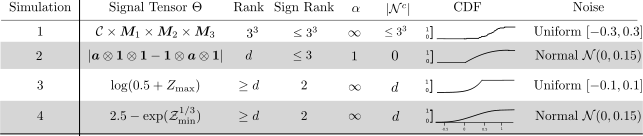
\includegraphics[width=1\textwidth]{figure/simulation.pdf}
\caption{Simulation models used for comparison. We use $\mM_k\in\{0,1\}^{d\times 3}$ to denote membership matrices, $\tC\in\mathbb{R}^{3\times 3\times 3}$ the block means, $\ma=d^{-1}(1,2,\ldots,d)^T \in\mathbb{R}^d$, $\tZ_{\max}$ and $\tZ_{\min}$ are order-3 tensors with entries $\max(i,j,k)/d$ and $\min(i,j,k)/d$, respectively.}\label{tab:simulation}
\end{table*}


Figure~\ref{fig:compare1} compares the estimation error under full observation. The MAE decreases with tensor dimension for all three methods. We find that our method {\bf NonParaT} achieves the best performance in all scenarios, whereas the second best method is {\bf CPT} for models 1-2, and {\bf NonParaM} for models 3-4. One possible reason is that models 1-2 have controlled multilinear tensor rank, which makes tensor methods {\bf NonParaT} and {\bf CPT} more accurate than matrix methods. For models 3-4, the rank exceeds the tensor dimension, and therefore, the two nonparametric methods {\bf NonParaT} and {\bf NonparaM} exhibit the greater advantage for signal recovery. 



Figure~\ref{fig:compare2} shows the completion error against observation fraction. We fix $d=40$ and gradually increase the observation fraction ${|\Omega|/d^3}$ from 0.3 to 1. We find that {\bf NonParaT} achieves the lowest error among all methods. Our simulation covers a reasonable range of  complexities; for example, model 1 has $3^3$ jumps in the CDF of signal $\Theta$, and models 2 and 4 have unbounded noise. Nevertheless, our method shows good performance in spite of model misspecification. This robustness is appealing in practice because the structure of underlying signal tensor is often unknown. 

\begin{figure}[h!]
\includegraphics[width=\textwidth]{figure/fig1-4v2.pdf}
\caption{Estimation error versus tensor dimension. Panels (a)-(d) correspond to simulation models 1-4 in Table~\ref{tab:simulation}.}\label{fig:compare1}
\end{figure}


\begin{figure}[h!]
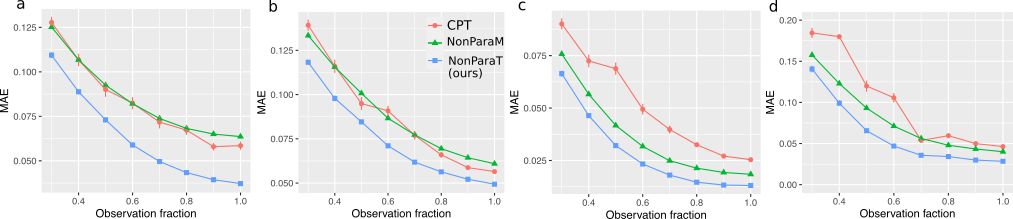
\includegraphics[width=\textwidth]{figure/fig5-8v2.pdf}
\caption{Completion error versus observation fraction. Panels (a)-(d) correspond to simulation models 1-4 in Table~\ref{tab:simulation}. }\label{fig:compare2}
\end{figure}



\subsection{Brain connectivity analysis}
We apply our method to two tensor datasets, the MRN-114 human brain connectivity data~\citep{wang2017bayesian}, and NIPS word occurrence data~\citep{globerson2007euclidean}. The first data tensor consists of binary entries only, and the second data tensor consists of continuous-valued entries. 

The brain dataset records the structural connectivity among 68 brain regions for 114 individuals along with their Intelligence Quotient (IQ) scores. We organize the connectivity data into an order-3 tensor, where entries encode the presence or absence of fiber connections between brain regions across individuals. 

\begin{figure}[h!]
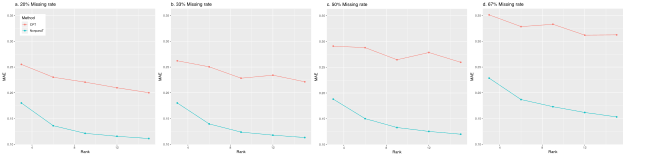
\includegraphics[width = \textwidth]{figure/brain_sim.pdf}
\caption{Estimation error versus rank under different missing rate. Panels (a)-(d) correspond to missing rate 20\%, 33\%, 50\%, and 67\%, respectively. Error bar represents the standard error over 5-fold cross-validations.}\label{fig:braincv}
\end{figure}

Figure~\ref{fig:braincv} shows the MAE based on 5-fold cross-validations with $r = 3,6,\ldots, 15$ and $H = 20$. We find that our method outperforms CPT in all combinations of ranks and missing rates. The achieved error reduction appears to be more profound as the missing rate increases. This trend highlights the applicability of our method in tensor completion tasks. In addition, our method exhibits a smaller standard error in cross-validation experiments as shown in Figure~\ref{fig:braincv} and Table~\ref{tab:data}, demonstrating the stability over CPT.  One possible reason is that that our estimate is guaranteed to be in $[0,1]$ (for probabilistic tensor estimation) whereas CPT estimation may fall outside the valid range $[0,1]$. 


\begin{table}[h!]
\centering
\resizebox{1\textwidth}{!}{
\begin{tabular}{c|c|c|c|c|c}
\Xhline{2\arrayrulewidth}
\multicolumn{6}{c}{MRN-114 brain connectivity dataset}\\
\Xhline{2\arrayrulewidth}
Method             &$r =3$        & $r=6$ &  $r=9$&$r=12$&$r = 15$\\
\hline
NonparaT (Ours)& ${\bf 0.18}(0.001)$ &$ {\bf 0.14}(0.001)$ & ${\bf 0.12}(0.001)$&${\bf 0.12}(0.001)$&${\bf 0.11}(0.001)$\\
Low-rank CPT &$0.26(0.006)$ & $0.23(0.006$)&$0.22(0.004)$&$0.21(0.006)$&$0.20(0.008)$\\
 \Xhline{2\arrayrulewidth}
 \multicolumn{6}{c}{NIPS word occurrence dataset}\\
 \Xhline{2\arrayrulewidth}
Method             &$r =3$        & $r=6$ &  $r=9$&$r=12$&$r = 15$\\
\hline
NonparaT (Ours) & ${\bf 0.18}(0.002)$ & ${\bf 0.16}(0.002)$ & ${\bf 0.15}(0.001)$& ${\bf 0.14}(0.001)$&${\bf 0.13}(0.001)$\\
 \hline
Low-rank CPT &$0.22(0.004)$ & $0.20(0.007)$ & $0.19(0.007)$&$0.17(0.007)$&$0.17(0.007)$\\
  \hline
Naive imputation (Baseline)& \multicolumn{5}{c}{$0.32(.001)$}
\end{tabular}
}
\caption{MAE comparison in the brain data and NIPS data analysis. Reported MAEs are averaged over five runs of cross-validation, with 20\% entries for testing and 80\% for training, with standard errors in parentheses. Bold numbers indicate the minimal MAE among three methods. For low-rank CPT, we use R function {\tt rTensor} with default hyperparameters, and for our method, we set $H=20$.}\label{tab:data}
\end{table}

We next investigate the pattern in the estimated signal tensor. Figure~\ref{fig:signal}a shows the identified top edges associated with IQ scores. Specifically, we first obtain a denoised tensor $\hat \Theta\in\mathbb{R}^{68\times 68\times 114}$ using our method with $r=10$ and $H=20$. Then, we perform a regression analysis of $\hat \Theta(i,j,\colon)\in\mathbb{R}^{144}$ against the normalized IQ score across the 144 individuals. The regression model is repeated for each edge $(i,j)\in[68]\times[68]$. We find that top edges represent the interhemispheric connections in the frontal lobes.  The result is consistent with recent research on brain connectivity with intelligence~\citep{li2009brain,wang2017bayesian}.



\subsection{NIPS data analysis}

The NIPS dataset consists of word occurrence counts in papers published from 1987 to 2003. We focus on the top 100 authors, 200 most frequent words, and normalize each word count by log transformation with pseudo-count 1. The resulting dataset is an order-3 tensor with entry representing the log counts of words by authors across years. 


Table~\ref{tab:data} compares the prediction accuracy of different methods. We find that our method substantially outperforms the low-rank CP method for every configuration under consideration. Further increment of rank appears to have little effect on the performance. 
The comparison highlights the advantage of our method in achieving accuracy while maintaining low complexity. In addition, we also perform naive imputation where the missing values are predicted using the sample average. Both our method and CPT outperform the naive imputation, implying the necessity of incorporating tensor structure in the analysis.

\begin{figure}[h!]
\centering
\includegraphics[width=.39\textwidth]{figure/brainIQ.pdf}
\hspace{1cm}
\includegraphics[width=.495\textwidth]{figure/signal.pdf}
\caption{Estimated signal tensors in the data analysis. (a) top edges associated with IQ scores in the brain connectivity data. The color indicates the estimated IQ effect size. (b) top authors and words for years 1996-1999 in the NIPS data. Authors and words are ranked by marginal averages based on $\hat \Theta$, where the marginal average is denoted in the parentheses.
}\label{fig:signal}
\end{figure}


We next examine the estimated signal tensor $\hat \Theta$ from our method.  Figure~\ref{fig:signal}b illustrates the results from NIPS data, where we plot the entries in $\hat \Theta$ corresponding to top authors and most-frequent words (after excluding generic words such as \emph{figure}, \emph{results}, etc). The identified pattern is consistent with the active topics in the NIPS publication. Among the top words are \emph{neural} (marginal mean = 1.95), \emph{learning} (1.48), and \emph{network} (1.21), whereas top authors are \emph{T.\ Sejnowski} (1.18), \emph{B.~Scholkopf} (1.17), \emph{M.\ Jordan} (1.11), and \emph{G.\ Hinton} (1.06). We also find strong heterogeneity among word occurrences across authors and years. For example, \emph{training} and \emph{algorithm} are popular words for \emph{B.\ Scholkopf} and \emph{A.\ Smola} in 1998-1999, whereas \emph{model} occurs more often in \emph{M.\ Jordan} and in 1996. The detected pattern and achieved accuracy demonstrate the applicability of our method.




\section{Discussion}\label{sec:conclusion}
We have developed a tensor estimation method that addresses both low- and high-rankness based on
sign series representation. Our work provides a nonparametric framework for tensor estimation, and
we establish accuracy guarantees for recovering a wide range of structured tensors. Our proposed
learning-reduction strategy empowers existing algorithms for broader implication, thereby connecting
the low-rank (parametric) tensors and high-rank (nonparametric) tensors. We hope the work opens up
new inquiry that allows more researchers to contribute to this field.


There are several possible extensions from our work. In our theory, we assume the true sign-rank $r$ is known or otherwise has been consistently estimated; the adaptivity to unknown $r$ is empirically addressed by cross-validation. In principle, a larger $r$ leads to a smaller approximation bias but a larger estimation variance; vice versa for a smaller $r$. When we set the rank smaller than true signal rank $r$, this would incur extra approximation bias. The level of approximation bias depends on the spectral complexity of the signal tensor. In the matrix case, the approximation bias is well quantified by tail eigenvalues; however, such extension to higher-order tensors is known to be very challenging, partly due to lack of spectral theory. We will leave the optimality of unknown rank as future research.


Exploring the minimax nonparametric rate among polynomial-time tensor algorithms warrants future work. In the special setting of tensor order $K = 2$ (i.e.\ matrix case) with smoothness $\alpha=1$, our method achieves the error rate $\tilde\tO(d^{-(K-1)/3})$. This rate agrees with RMSE rate obtained by Lipschitz graphon model~\citep{xu2018rates}. It has been conjectured that $\tilde \tO(d^{-1/3})$ is the best computationally efficient rate for $K=2$~\citep{xu2018rates,zhang2018network}. We conjecture the similar phenomenon extends to higher-order tensors $(K\geq 3)$; a full exploration will be the future work. 

Our model is related to but distinct from simple hypergraphons~\citep{balasubramanian2021nonparametric} as mentioned in Remark~\ref{rmk:graphon}. 
The improvement of our approach over simple smooth hypergraphon bears the analogy of Lebesque vs.\ Riemann integrals in functional analysis. In addition, simple hypergraphon uses random design points, whereas our example uses deterministic design points. These two choices of designs lead to a notable different analysis in the same spirit as random- vs. fixed-designs in nonparametric regression. Whether it is possible to extend our theory to general hypergraphon is an interesting question for future research.

Finally, our learning-reduction algorithm uses evenly spaced grid of levels, $\tH=\{-1,\ldots,-1/H,$ $0, 1/H,\ldots,1\}$. Our theory continues to hold true for non-evenly spaced grids, as long as the spacings converge at a same rate. In principle, using non-evenly spaced grid may improve the local adaptivity, and we conjecture that the optimal grid design depends on the true (but unknown) shape of the CDF $G(\cdot)$. In real applications, however, we usually have no prior information on function smoothness of $\alpha$. The lack of prior knowledge makes optimal grid design sensitive to model misspecification. Therefore, we choose to present the evenly spaced grid to achieve a good balance between theory and empirical applicability. 

\section*{Acknowledgements}
This research is supported in part by NSF CAREER DMS-2141865, NSF grant DMS-1915978, DMS-2023239 and Wisconsin Alumni Research Foundation.





\appendix


\section{Experimental details in Section~\ref{sec:motivation}}\label{sec:numericalrank}
In Section~\ref{sec:motivation} of the main paper, we have provided a motivating example to show the sensitivity of tensor rank to monotonic transformations. Here, we describe the details of the experiment set-up. 

The step 1 is to generate a rank-3 tensor $\tZ$ based on the CP representation
\[
\tZ=\ma^{\otimes 3}+\mb^{\otimes 3}+\mc^{\otimes 3},
\]
where $\ma,\mb,\mc\in\mathbb{R}^{30}$ are vectors consisting of $N(0,1)$ entries, and the shorthand $\ma^{\otimes 3}=\ma\otimes \ma\otimes \ma$ denotes the Kronecker power. We then apply $f(z)=(1+\exp(-cz))^{-1}$ to $\tZ$ entrywise, and obtain a transformed tensor $\Theta=f(\tZ)$. 

The step 2 is to determine the rank of $\Theta$. Unlike matrices, the exact rank determination for tensors is NP hard. Therefore, we choose to compute the numerical rank of $\Theta$ as an approximation.  The numerical rank is determined as the minimal rank for which the relative approximation error is below $0.1$. We define two numerical ranks; CP and Tucker rank.
\begin{align}\label{eq:numeric}
& \widehat{\rank}(\Theta)=\min\left\{s\in\mathbb{N}_{+}\colon \min_{\hat \Theta\colon \rank(\hat \Theta)\leq s}{\FnormSize{}{\Theta-\hat \Theta}\over \FnormSize{}{\Theta}} \leq 0.1\right\}\\
& \widehat{\text{Tucker$-$rank}}(\Theta)=\min\left\{s\in\mathbb{N}_{+}\colon \min_{\hat \Theta\colon \text{Tucker-rank}(\hat \Theta)\leq (s,s,s)}{\FnormSize{}{\Theta-\hat \Theta}\over \FnormSize{}{\Theta}} \leq 0.1\right\}.
\end{align}
We compute $\hat r_{\text{cp}}(\Theta)$ by searching over $s\in\{1,\ldots,30^2\}$, where for each $s$, we (approximately) solve the least-square minimization using built-in \texttt{cp} function in R package {\tt rTensor} with default setting (iteration = 25, tolerance = $10^{-5}$). 
We compute $\hat r_{\text{tucker}}(\Theta)$ by searching over $s\in\{1,\ldots,30\}$ and solving the least-square minimization for each $s$ using built-in \texttt{tucker} function in R package {\tt rTensor} with default setting (iteration = 25, tolerance = $10^{-5}$). 
We repeat steps 1-2 ten times, and plot the averaged numerical rank of $\Theta$ versus transformation level $c$ in Figure~\ref{fig:example}a.  


\section{Proofs of theory in Section~\ref{sec:algebry}}\label{sec:proofalg}

\subsection{Proofs of Propositions~\ref{cor:monotonic}-\ref{prop:global2}}
\begin{proof}[Proof of Proposition~\ref{cor:monotonic}] 
\begin{enumerate}[label={2.\arabic*},wide, labelindent=0pt]
\item[Part (a).] By definition of sign-rank~\eqref{eq:sign-rank},
\[
\srank(\Theta-\pi)\leq \srank(\Theta)+\srank(\mathbf{1}\otimes \cdots \otimes \mathbf{1})=\srank(\Theta)+1\leq \rank(\Theta)+1.
\]
\item[Part (b).] The strict monotonicity of $g$ implies that the inverse function $g^{-1}\colon \mathbb{R}\to \mathbb{R}$ is well-defined. 
%Without loss of generality, assume $g(0)=0$, and it suffices to show 
%\begin{equation}\label{eq:shift}
%\srank(g(\Theta))\leq \rank(g(\Theta)).
%\end{equation}
%Otherwise, one can re-define $g'(x)\leftarrow g(x)-g(0)$. The shift changes left-hand-side of~\eqref{eq:shift} by at most 1, because $\rank(g'(\Theta))\leq \rank(g(\Theta))+1$. 

When $g$ is strictly increasing, the mapping $x\mapsto g(x)-g(0)$ is sign preserving. Specifically, if $x\geq 0$, then $g(x)\geq g(0)$. Conversely, if $g(x)\geq g(0)$, then applying $g^{-1}$ to both sides gives $x\geq 0$. 

When $g$ is strictly decreasing, the mapping $x\mapsto g(x)-g(0)$ is sign reversing. Specifically, if $x\geq 0$, then $g(x)\leq g(0)$. Conversely, if $g(x)\leq g(0)$, then applying $g^{-1}$ to both sides gives $x\leq 0$.

Combining the above two cases gives that $\Theta\simeq g(\Theta)-g(0)$ or $\Theta\simeq -(g(\Theta)-g(0))$. Since constant multiplication  does not change the tensor rank,  we have $\srank(\Theta)=\srank(g(\Theta)-g(0))\leq \rank (g(\Theta))+1$. 
\item[Part (c).] See Example~\ref{example:max} for constructive examples.
\end{enumerate}
\end{proof}

\begin{proof}[Proof of Proposition~\ref{prop:repeat}]
We reorder the tensor indices along each mode such that $x^{(k)}_{1}\leq \cdots \leq x^{(k)}_{d_k}$ for all $k\in[K]$. Based on the construction of $\tZ_{\max}$, the reordering does not change the rank of $\tZ_{\max}$ or $(\Theta-\pi)$. Let $z_1<\cdots<z_r$ be the $r$ distinct real roots for the equation $g(z)=\pi$. We separate the proof for two cases, $r=1$ and $r\geq 2$. 

\begin{itemize}[leftmargin=*,topsep=0pt,itemsep=-1ex,partopsep=1ex,parsep=1ex]
\item When $r=1$. The continuity of $g(\cdot)$ implies that the function $(g(z)-\pi)$ has at most one sign change point. Using similar proof as in Example~\ref{example:max}, we have
\begin{align}
&\sign(\Theta-\pi)=1-2\ma^{(1)}\otimes\cdots\otimes \ma^{(K)}\quad \text{ or } \quad \sign(\Theta-\pi) = 2\ma^{(1)}\otimes\cdots\otimes \ma^{(K)} -1,
\end{align}
where $\ma^{(k)}$ are binary vectors defined by
\[
\ma^{(k)}=(\KeepStyleUnderBrace{1,\ldots,1,}_{\text{positions for which $x_{i_k}^{k}<z_1$}}0,\ldots,0)^T, \quad \text{for }k\in[K].
\]
Therefore, $\srank(\Theta-\pi)\leq \rank(\sign(\Theta-\pi)) = 2$. 

\item When $r\geq 2$.   By continuity, the function $(g(z)-\pi)$ is non-zero and remains an unchanged sign in each of the intervals $(z_s, z_{s+1})$ for $1\leq s\leq r-1$. Define the index set 
\[
\tI=\{s\in\mathbb{N}_{+}\colon \text{the interval $(z_s, z_{s+1})$ in which $g(z)<\pi$}\}.
\] 
We now prove that the sign tensor $\sign(\Theta-\pi)$ has rank bounded by $2r-1$. To see this, consider the tensor indices for which $\sign(\Theta-\pi)=-1$,
\begin{align}\label{eq:support}
\{\omega\colon \Theta(\omega)-\pi <0 \} & = \{\omega \colon g(\tZ_{\max}(\omega))<\pi\} \notag \\
&=\cup_{s\in \tI} \{\omega\colon \tZ_{\max}(\omega)\in(z_s,z_{s+1})\}\notag\\
&=\cup_{s\in \tI}\Big( \{\omega\colon \text{$x^{(k)}_{i_k}< z_{s+1}$ for all $k\in[K]$}\}\cap \{\omega\colon \text{$x^{(k)}_{i_k}\leq z_{s}$ for all $k\in[K]$}\}^c\Big).
\end{align}
The equation~\eqref{eq:support} is equivalent to 
\begin{align}\label{eq:indicator}
\mathds{1}(\Theta(i_1,\ldots,i_K)< \pi)&
=\sum_{s\in \tI}\left( \prod_k \mathds{1}(x^{(k)}_{i_k}< z_{s+1}) - \prod_k \mathds{1}(x^{(k)}_{i_k}\leq z_{s})\right),
\end{align}
for all $(i_1,\ldots,i_K)\in[d_1]\times \cdots\times[d_K]$, where $\mathds{1}(\cdot)\in\{0,1\}$ denotes the indicator function. The equation~\eqref{eq:indicator} implies the low-rank representation of $\sign(\Theta-\pi)$,
\begin{equation}\label{eq:sum}
\sign(\Theta-\pi)=1-2\sum_{s\in \tI } \left(\ma^{(1)}_{s+1}\otimes\cdots\otimes \ma^{(K)}_{s+1} - \bar \ma^{(1)}_s\otimes\cdots\otimes \bar \ma^{(K)}_s\right),
\end{equation}
where $\ma^{(k)}_{s+1}, \ma^{(k)}_{s}$ are binary vectors defined by
\[
\ma^{(k)}_{s+1}=(\KeepStyleUnderBrace{1,\ldots,1,}_{\text{positions for which $x_{i_k}^{(k)}<z_{s+1}$}}0,\ldots, 0)^T,\quad \text{and}\quad
\bar \ma^{(k)}_s=(\KeepStyleUnderBrace{1,\ldots,1,}_{\text{positions for which $x_{i_k}^{(k)}\leq z_{s}$}}0,\ldots, 0)^T.
\]
Therefore, by~\eqref{eq:sum} and the assumption $|\tI|\leq r-1$, we conclude that 
\[
\srank(\Theta-\pi)\leq 1+2(r-1)=2r-1.
\]
\end{itemize}
Combining two cases yields that $\srank(\Theta-\pi)\leq 2r$ for any $r\geq 1$.
\end{proof}


\begin{proof}[Proof of Proposition~\ref{prop:connection}]
The conclusion directly follows from the definition of tensor rank. 
\end{proof}


\begin{proof}[Proof of Example~\ref{example:max}]
We first prove the results for $K=2$. The full-rankness of $\Theta$ is verified from elementary row operations as follows
\begin{align}
\begin{pmatrix}
(\Theta_2-\Theta_1)/(\log(1+\frac{2}{d})-\log(1+\frac{1}{d}))\\(\Theta_3-\Theta_2)/(\log(1+\frac{3}{d})-\log(1+\frac{2}{d}))\\\vdots\\ (\Theta_d-\Theta_{d-1})/(\log(1+\frac{d}{d})-\log(1+\frac{d-1}{d}))\\\Theta_d/\log(1+\frac{d}{d})
\end{pmatrix} = \begin{pmatrix}
 1&          0  &      \ddots  &        \ddots       &          0 \\
1& 1 & \ddots &            \ddots   &   \ddots          \\
      \vdots &     \vdots & \ddots &       \ddots &    \ddots         \\
 1 & 1 &1 & 1 &0\\
 1 & 1 &1 & 1 &1
\end{pmatrix},
\end{align}
where $\Theta_i$ denotes the $i$-th row of $\Theta$. 
Now it suffices to show $\srank(\Theta-\pi)\leq 2$ for $\pi$ in the feasible range $(\log(1+{1\over d}),\ \log 2)$. In this case, there exists an index $i^*\in\{2,\ldots,d\}$, such that $\log(1+{i^*-1\over d})< \pi\leq \log(1+{i^*\over d})$. By definition, the sign matrix $\sign (\Theta-\pi)$ takes the form
\begin{equation}\label{eq:matrix}
\sign (\Theta(i,j)-\pi)=
\begin{cases}
-1, & \text{both $i$ and $j$ are smaller than $i^*$};\\
1, & \text{otherwise}.
\end{cases}
\end{equation}
Therefore, the matrix $\sign (\Theta-\pi)$ is a rank-2 block matrix, which implies $\srank(\Theta-\pi)=2$. 

We now extend the results to $K\geq 3$. By definition of the tensor rank, the rank of a tensor is lower bounded by the rank of its matrix slice.  So we have $\rank(\Theta)\geq \rank(\Theta(\colon,\colon,1,\ldots,1))=d$. For the sign-rank with feasible $\pi$, notice that the sign tensor $\sign(\Theta-\pi)$ takes the similar form as in~\eqref{eq:matrix},
\begin{equation}\label{eq:entrywise}
\sign (\Theta(i_1,\ldots,i_K)-\pi)=
\begin{cases}
-1, & \text{$i_k<i^*$ for all $k\in[K]$};\\
1, & \text{otherwise},
\end{cases}
\end{equation}
where $i^*$ denotes the index that satisfies $\log(1+\frac{i^*-1}{d})<\pi\leq \log(1+\frac{i^*}{d})$.
The equation~\eqref{eq:entrywise} implies that $\sign(\Theta-\pi)=-2\ma^{\otimes K}+1$, where $\ma=(1,\ldots,1,0,\ldots,0)^T$ takes 1 on the $i$-th entry if $i<i^*$ and 0 otherwise. Henceforth $\srank(\Theta-\pi)=2$. 
\end{proof}
\begin{rmk}
Example~\ref{eq:example} is proved in the similar way.
\end{rmk}




\begin{proof}[Proof of Example~\ref{example:banded}]
Note that $\mM$ is a banded matrix with entries
\[
\mM(i,j)={|i-j|}, \quad \text{for all }(i,j)\in[d]^2.
\]
Elementary row operation shows that $\mM$ is full rank as follows,
\begin{align}
\begin{pmatrix}
(\mM_1+\mM_d)/(d-1)\\
\mM_1-\mM_2\\
\mM_2-\mM_3\\
\vdots\\
\mM_{d-1}-\mM_{d}
\end{pmatrix} = 
\begin{pmatrix}
1&1&1&\cdots&1&1\\
-1&1&1&\cdots&1&1\\
-1&-1&1&\cdots&1&1\\
\vdots & \vdots & \vdots & \vdots & \vdots & \vdots\\
-1&-1&-1&\cdots&-1&1
\end{pmatrix}.
\end{align}

We now show $\srank(\mM-\pi)\leq 3$ by construction. Define two vectors $\mb=(2^{-1},2^{-2},\ldots,2^{-d})^T\in\mathbb{R}^d$ and $\text{rev}(\mb)=(2^{-d},\ldots,2^{-1})^T\in\mathbb{R}^d$. We construct the following matrix
\begin{equation}\label{eq:A}
\mA=\mb\otimes\text{rev}(\mb)+\text{rev}(\mb)\otimes\mb.
\end{equation}
The matrix $\mA\in\mathbb{R}^{d\times d}$ is banded with entries
\[
\mA(i,j)=\mA(j,i)=\mA(d-i,d-j)=\mA(d-j,d-i)=2^{-d-1}\left(2^{j-i}+2^{i-j}\right),\ \text{for all }(i,j)\in[d]^2.
\] 
Furthermore, the entry value $\mA(i,j)$ decreases with respect to $|i-j|$; i.e., 
\begin{equation}\label{eq:decrease}
\mA(i,j) \geq \mA(i',j'), \quad \text{for all }|i-j|\geq |i'-j'|.
\end{equation}
Notice that for a given $\pi\in\mathbb{R}$, there exists $\pi'\in\mathbb{R}$ such that $\sign(\mA-\pi')=\sign(\mM-\pi)$. This is because both $\mA$ and $\mM$ are banded matrices satisfying monotonicity~\eqref{eq:decrease}. By definition~\eqref{eq:A}, $\mA$ is a rank-2 matrix. Henceforce, $\srank(\mM-\pi)=\srank(\mA-\pi')\leq 3.$
\end{proof}



%\begin{example}[Stacked identity matrices]\label{ex:identity}
%Let $\mI$ be a $d$-by-$d$ identity matrix. Then
%\[
%\rank(\mI)=d,\quad\text{and}\quad  \srank(\mI-\pi)\leq 3 \ \text{for all }\pi\in\mathbb{R}.
%\]
%\end{example}
%\begin{proof}[Proof of Example~\ref{ex:identity}]
%Depending on the value of $\pi$, the sign matrix $\sign(\mI-\pi)$ falls into one of the two cases: 
%\begin{enumerate}
%\item[(a)] $\sign(\mI-\pi)$ is a matrix of all $1$, or of all $-1$; 
%\item[(b)] $\sign(\mI-\pi)=2\mI-\mathbf{1}_d\otimes \mathbf{1}_d$.
%\end{enumerate}
%The first cases are trivial, so it suffices to show $\srank(\mI-\pi)\leq 3$ in the third case.   


%Based on Example~\ref{example:banded}, the rank-2 matrix $\mA$ in~\eqref{eq:A} satisfies 
%\[
%\mA(i,j)
%\begin{cases}
%=2^{-d}, & i=j,\\
%\geq 2^{-d}+2^{-d-2}, & i\neq j.
%\end{cases}
%\]
%Therefore, $\sign\left(2^{-d}+2^{-d-3}-\mA\right)=2\mI-\mathbf{1}_d\otimes \mathbf{1}_d$. We conclude that $\srank(\mI-\pi)\leq \rank(2^{-d}+2^{-d-3}-\mA)=3$. 
%\end{proof}




\section{Proofs of Theory in Section~\ref{sec:stat}}\label{sec:proofs}
\subsection{Proof of Theorem~\ref{prop:global}}
\begin{proof}[Proof of Theorem~\ref{prop:global}]
Fix $\pi\in[-1,1]$. Denote $\bar \Theta=(\Theta-\pi)$ and $\bar \tY=(\tY-\pi)$. Based on the definition of classification loss $L(\cdot,\cdot)$, the function $\risk(\cdot)$ relies only on the sign pattern of the tensor. Therefore, without loss of generality, we assume both $\bar \Theta, \tZ \in\{-1,1\}^{d_1\times \cdots \times d_K}$ are binary tensors. 
We evaluate the excess risk 
\begin{equation}\label{eq:risk}
\risk(\tZ)- \risk(\bar \Theta) = \mathbb{E}_{\omega\sim \Pi}\KeepStyleUnderBrace{\mathbb{E}_{\tY(\omega)}\left\{|\tY(\omega)-\pi|\left[\left|\tZ(\omega)-\sign(\bar \tY(\omega)) \right|-\left|\bar\Theta(\omega)-\sign(\bar \tY(\omega))\right|\right]\right\}}_{\stackrel{\text{def}}{=}I(\omega)}.
\end{equation}
Denote $y=\tY(\omega)$, $z=\tZ(\omega)$, $\bar \theta=\bar\Theta(\omega)$, and $\theta=\Theta(\omega)$. The expression of $I(\omega)$ is simplified as
\begin{align}\label{eq:I}
I(\omega)&= \mathbb{E}_{y|\omega}\left[ (y-\pi)(\bar \theta-z)\mathds{1}(y\geq \pi)+(\pi-y)(z-\bar \theta)\mathds{1}(y< \pi)\right]\notag \\
&= \mathbb{E}_{y|\omega}\left[(\bar \theta-z) (y-\pi)\right]\notag \\
&=  \left[\sign(\theta-\pi)-z\right]\left(\theta-\pi\right)\notag \\
&= |\sign(\theta-\pi)-z||\theta-\pi|\geq 0,
\end{align}
where the third line uses the fact $\mathbb{E}y=\theta$ and $\bar \theta=\sign(\theta-\pi)$, and the last line uses the assumption $z \in\{-1,1\}$. The equality~\eqref{eq:I} is attained when $z=\sign(\theta-\pi)$ or $\theta=\pi$. Combining~\eqref{eq:I} with~\eqref{eq:risk}, we conclude that, for all $\tZ\in\{-1,1\}^{d_1\times \cdots \times d_K}$, 
\begin{equation}\label{eq:minimum}
\risk(\tZ)- \risk(\bar \Theta) = \mathbb{E}_{\omega\sim \Pi} |\sign(\Theta(\omega)-\pi)-\tZ(\omega)||\Theta(\omega)-\pi|\geq 0.
\end{equation}
In particular, setting $\tZ=\bar \Theta=\sign(\Theta-\pi)$ in~\eqref{eq:minimum} yields the minimum. Therefore, 
\[
\risk(\bar \Theta)=\min\{\risk(\tZ)\colon \tZ\in \mathbb{R}^{d_1\times \cdots \times d_K}\} \leq \min\{\risk(\tZ)\colon \rank(\tZ)\leq r\}.
\]
Since $\srank(\Theta-\pi)\leq r$ by assumption, the last inequality becomes equality. The proof is complete. 
\end{proof}

\subsection{Proof of Theorem~\ref{thm:population}}
\begin{proof}[Proof of Theorem~\ref{thm:population}]
Fix $\pi\notin\tN$ and denote $\bar \Theta=(\Theta-\pi)$. Based on~\eqref{eq:minimum} in Theorem~\ref{prop:global}, we have
\begin{equation}\label{eq:population2}
\risk(\tZ)- \risk(\bar \Theta) = \mathbb{E}\left[|\sign \tZ-\sign\bar \Theta||\bar \Theta|\right].
\end{equation}
The Definition~\ref{ass:margin} states that
\begin{align}\label{eq:ass}
\mathbb{P}\left(|\bar \Theta | \leq t\right) \leq 
\begin{cases}ct^\alpha, & \text{for all } \Delta s \leq t< \rho(\pi,\tN),\\
C\Delta s, & \text{for all }0\leq t< \Delta s.
\end{cases}
\end{align}
Without further specification, all relevant probability statements, such as $\mathbb{E}$ and $\mathbb{P}$, are with respect to $\omega\sim \Pi$. 

We divide the proof into two cases: $\alpha >0$ and $\alpha = \infty$.
\begin{itemize}[leftmargin=*,topsep=0pt,itemsep=-1ex,partopsep=1ex,parsep=1ex]
\item Case 1: $\alpha>0$. 

By~\eqref{eq:population2}, for all $0 \leq t< \rho(\pi, \tN)$,
\begin{align}\label{eq:1}
\risk(\tZ)- \risk(\bar \Theta) &\geq t\mathbb{E}\left(|\sign \tZ- \sign \bar\Theta|\mathds{1}\{|\bar\Theta|>t\}\right)
\notag \\
&\geq 2t\mathbb{P}\left(\sign\tZ \neq \sign \bar \Theta\text{ and }|\bar \Theta|>t   \right)\notag \\
& \geq 2t\Big\{\mathbb{P}\left(\sign\tZ \neq \sign \bar \Theta \right) - \mathbb{P}\left(|\bar \Theta|\leq t\right)\Big\}\notag\\
&\geq t\Big\{\textup{MAE}(\sign \tZ, \sign \bar \Theta) - C\Delta s - 2ct^\alpha \Big\},
\end{align}
where the last line follows from the definition of MAE and~\eqref{eq:ass}. We maximize the lower bound~\eqref{eq:1} with respect to $t$, and obtain the optimal $t_{\text{opt}}$,
\[
t_{\text{opt}}=\begin{cases}
\rho(\pi, \tN), & \text{if } \textup{MAE}(\sign \tZ,\sign \bar\Theta) > \text{cut-off},\\
\left[ {1\over 2c(1+\alpha)} (\textup{MAE} (\sign \tZ,\sign \bar\Theta)-C\Delta S  )\right]^{1/\alpha}, &  \text{if }\textup{MAE}( \sign \tZ,\sign \bar\Theta) \leq \text{cut-off}.
 \end{cases}
\]
where we have denoted the cut-off $= 2c(1+\alpha) \rho^{\alpha}(\pi, \tN)+C\Delta s$.
%Notice that we use the fact $\textup{MAE} (\sign \tZ,\sign \bar\Theta)\gg \Delta s$ here. 
The corresponding lower bound of the inequality~\eqref{eq:1} becomes
\[
\risk(\tZ)- \risk(\bar \Theta) \geq 
\begin{cases}
c_1 \rho(\pi, \tN) \left[\textup{MAE}(\sign \tZ,\sign \bar\Theta)-C\Delta s\right],  & \text{if } \textup{MAE}(\sign \tZ,\sign \bar\Theta) > \text{cut-off},\\
c_2 \left[ \textup{MAE}( \sign \tZ,\sign \bar\Theta)-C\Delta s\right]^{1+\alpha \over \alpha}, & \text{if }\textup{MAE}(\sign \tZ,\sign \bar\Theta) \leq \text{cut-off},
\end{cases}
\]
where $c_1,c_2>0$ are two constants independent of $\tZ$. Combining both cases gives
\begin{align}\label{eq:MAE}
\textup{MAE}(\sign \tZ,\sign \bar\Theta) & \lesssim [\risk(\tZ)- \risk(\bar \Theta)]^{\alpha\over 1+\alpha}+{1\over \rho(\pi, \tN)} \left[\risk(\tZ)- \risk(\bar \Theta)\right]+\Delta s\\
&\leq C(\pi)[\risk(\tZ)- \risk(\bar \Theta)]^{\alpha\over 1+\alpha}+\Delta s,
\end{align}
where $C(\pi)>0$ is a multiplicative factor independent of $\tZ$. 
\item Case 2: $\alpha=\infty$. The inequality~\eqref{eq:1} now becomes
\begin{equation}\label{eq:2}
\risk(\tZ)- \risk(\bar \Theta) \geq t\left[\textup{MAE}(\sign \bar\Theta, \sign \tZ)-C\Delta s\right], \quad \text{for all }0\leq t< \rho(\pi,\tN).
\end{equation}
The conclusion follows by taking $t={\rho(\pi, \tN)\over 2}$ in the inequality~\eqref{eq:2}. 
\end{itemize}
\end{proof}
\begin{rmk}\label{eq:rmk}The proof of Theorem~\ref{thm:population} shows that, under global $\alpha$-smoothness of $\Theta$, 
\begin{equation}\label{eq:remark}
\textup{MAE}(\sign \tZ,\sign \bar \Theta)  \lesssim [\risk(\tZ)- \risk(\bar \Theta)]^{\alpha\over 1+\alpha}+{1\over \rho(\pi, \tN)} \left[\risk(\tZ)- \risk(\bar \Theta)\right]+\Delta s,
\end{equation}
for all $\tZ\in\mathbb{R}^{d_1\times \cdots \times d_K}$. For fixed $\pi$, the second term is absorbed into the first term. 
\end{rmk}



\subsection{Proof of Theorem~\ref{prop:global2}}
\begin{proof}[Proof of Theorem~\ref{prop:global2}]
Denote $\bar \Theta=(\Theta-\pi)$ and $\bar \tY=(\tY-\pi)$. Similar to the proof of Theorem~\ref{prop:global}, we evaluate the excess risk 
\begin{equation}\label{eq:risk}
\risk_q(\tZ)- \risk_q(\bar \Theta) = \mathbb{E}_{\omega\sim \Pi}\KeepStyleUnderBrace{\mathbb{E}_{\tY(\omega)}\left\{|\tY(\omega)-\pi|^q\left[\left|\tZ(\omega)-\sign(\bar \tY(\omega)) \right|-\left|\bar\Theta(\omega)-\sign(\bar \tY(\omega))\right|\right]\right\}}_{\stackrel{\text{def}}{=}I(\omega)}.
\end{equation}
The expression of $I(\omega)$ is simplified as
\begin{align}\label{eq:I_q}
I(\omega)&= \mathbb{E}_{\tY(\omega)\geq \pi}\left[ (\tY(\omega)-\pi)^q(\sign(\bar \Theta(\omega))-\sign(\tZ(\omega)))\right]\\&\hspace{2cm}+\mathbb{E}_{\tY(\omega)< \pi}\left[ (\pi-\tY(\omega))^q(\sign(\tZ(\omega))-\sign(\bar \Theta(\omega)))\right].
\end{align}
We consider two cases when $q$ is an odd number and an even number.
\begin{itemize}[leftmargin=*,topsep=0pt,itemsep=-1ex,partopsep=1ex,parsep=1ex]
    \item Case 1: $q$ is an odd number. In this case, $I(\omega)$ becomes
    \begin{align}
        I(\omega)  &=  \mathbb{E}_{\tY(\omega)}\left[(\tY(\omega)-\pi)(\sign(\bar\Theta(\omega))-\sign(\tZ(\omega)))\right]\\&=
        \left(\sign(\bar\Theta(\omega))-\sign(\tZ(\omega))\right)\mathbb{E}_{\tY(\omega)}\left[\tY(\omega)-\pi\right]^q
    \end{align}
    Therefore, $I(\omega)$ is minimized when
    \begin{align}\label{eq:oddt}
        \sign(\tZ(\omega)) = \sign(\mathbb{E}_{\tY(\omega)}\left(\tY(\omega)-\pi)^q\right).
    \end{align}
    Denote $y=\tY(\omega)$, $\theta = \Theta(\omega)$, and $\tE(\omega) = \epsilon$.
    Under the condition that $\epsilon$ is symmetric zero-mean noise, we show that
    \begin{align}\label{eq:odd}
        \sign\left(\mathbb{E}_y(y-\pi)^q\right) = \sign(\theta-\pi).
    \end{align}
    Notice that 
    \begin{align}
        \mathbb{E}_y(y-\pi)^q & = \sum_{k = 0}^q {q\choose k}(\theta-\pi)^{p-k}\mathbb{E}_y(y-\theta)^k\\&= \sum_{k=0}^{(p-1)/2}(\theta-\pi)^{p-2k}\mathbb{E}\epsilon^{2k},
    \end{align}
    where the last line uses the noise distribution is symmetric about the  origin. Therefore, we prove  \eqref{eq:odd}.
    
    \item Case 2: $q$ is an even number. In this case, $I(\omega)$ becomes
    \begin{align}
         I(\omega)  &=  
        \left(\sign(\bar\Theta(\omega))-\sign(\tZ(\omega))\right)\left(\mathbb{E}_{\tY(\omega)\geq \pi}\left[\tY(\omega)-\pi\right]^q-\mathbb{E}_{\tY(\omega)< \pi}\left[\tY(\omega)-\pi\right]^q\right).
    \end{align}
    Therefore, $I(\omega)$ is minimized when
    \begin{align}\label{eq:event}
        \sign(\tZ(\omega)) = \sign\left(\mathbb{E}_{\tY(\omega)\geq \pi}\left[\tY(\omega)-\pi\right]^q-\mathbb{E}_{\tY(\omega)< \pi}\left[\tY(\omega)-\pi\right]^q\right).
    \end{align}
    Denote $y=\tY(\omega)$, $\theta = \Theta(\omega)$, and $\tE(\omega) = \epsilon$.
    Under the condition that $\epsilon$ is symmetric zero-mean noise, we show that
    \begin{align}\label{eq:even}
        \sign\left(\mathbb{E}_{y-\pi\geq 0}\left(y-\pi\right)^q-\mathbb{E}_{y-\pi<0}\left(y-\pi\right)^q\right) = \sign(\theta-\pi).
    \end{align}
    Let $x := y-\pi = \theta-\pi+\epsilon$. Notice that $x$ is a random variable which is symmetric at $m:= \theta-\pi$. First suppose $m\geq0$, then we have
    \begin{align}
      \mathbb{E}_{y-\pi\geq 0}\left(y-\pi\right)^q-\mathbb{E}_{y-\pi<0}\left(y-\pi\right)^q &=  \int_{x\geq 0}x^qdx-\int_{x<0}x^qdx\\&\geq \int_{x\geq m}x^qdx-\int_{x<m}x^qdx \\&=\int_{x\geq m}\sum_{k=0}^q{q\choose k}(x-m)^k m^{p-k}dx\\&\hspace{2cm}-\int_{x<m}\sum_{k=0}^q{q\choose k}(x-m)^{k}m^{p-k}dx\\&= 2\int_{x\geq m}\sum_{k=0}^{q/2-1}{q\choose 2k+1}(x-m)^{2k+1}m^{p-2k-1}\\&\geq 0,
    \end{align}
    where the last equality uses the symmetry of $x$ around $m$. We can prove the case $m<0$ in the same way.
    Therefore, we show that \eqref{eq:event} holds true.
 
\end{itemize}
\end{proof}




\section{Proof of Theory in Section~\ref{sec:estimation}}\label{sec:novalty}

\subsection{Proof of sign tensor estimation}
The following lemma provides the variance-to-mean relationship implied by the $\alpha$-smoothness of $\Theta$. The relationship plays a key role in determining the convergence rate based on empirical process theory~\citep{shen1994convergence}; also see Theorem~\ref{thm:refer}.

\begin{lem}[Variance-to-mean relationship]\label{lem:variance}
Consider the same setup as in Theorem~\ref{thm:estimation}. Fix $\pi\notin \tN$. Let $L(\tZ, \bar Y_\Omega)$ be the $l_1$ weighted classification loss
\begin{align}\label{eq:sample2}
L(\tZ, \bar \tY_\Omega)&= {1\over |\Omega|}\sum_{\omega \in \Omega}\ \KeepStyleUnderBrace{|\bar \tY(\omega)|}_{\text{$l_1$ weight}}\  \times \ \KeepStyleUnderBrace{| \sign \tZ(\omega)-\sign \bar \tY(\omega)|}_{\text{classification loss}}\notag \\
&={1\over |\Omega|}\sum_{\omega \in \Omega}\ell_\omega(\tZ, \bar \tY),
\end{align}
where we have denoted the function $\ell_\omega(\tZ,\bar \tY)\stackrel{\text{def}}{=}|\bar \tY(\omega)||\sign\tZ(\omega)-\sign \bar \tY(\omega)|$. Under Definition~\ref{ass:margin} of the $\alpha$-smoothness of $\Theta$, we have
\begin{equation}\label{eq:variance}
\textup{Var}[\ell_\omega(\tZ,\bar \tY_{\Omega})-\ell_\omega(\bar \Theta, \bar \tY_\Omega)]\lesssim [\textup{Risk}(\tZ)-\textup{Risk}(\bar \Theta)]^{\alpha \over 1+\alpha}+{1\over \rho(\pi, \tN)}[\textup{Risk}(\tZ)-\textup{Risk}(\bar \Theta)]+\Delta s,
\end{equation}
for all tensors $\tZ\in\mathbb{R}^{d_1\times \cdots \times d_K}$. Here the expectation and variance are taken with respect to both $\tY(\omega)$ and $\omega\sim \Pi$. 
\end{lem}
\begin{proof}[Proof of Lemma~\ref{lem:variance}]
We expand the variance by
\begin{align}\label{eq:mae}
\text{Var}[\ell_\omega(\tZ,\bar \tY_\Omega)-\ell_\omega(\bar \Theta, \bar \tY_\Omega)] &\lesssim \mathbb{E}|\ell_\omega(\tZ,\bar \tY_\Omega)-\ell_\omega(\bar \Theta, \bar \tY_\Omega)|^2\notag \\
&\lesssim \mathbb{E}|\ell_\omega(\tZ,\bar \tY_\Omega)-\ell_\omega(\bar \Theta, \bar \tY_\Omega)|\notag \\
&\leq \mathbb{E}|\sign\tZ-\sign \bar \Theta| = \textup{MAE}(\sign\tZ, \sign \bar \Theta),
\end{align}
where the second line comes from the boundedness of classification loss $L(\cdot ,\cdot)$, and the third line comes from the inequality $||a-b|-|c-b||\leq |a-b|$ for $a,b,c\in\{-1,1\}$, together with the boundedness of classification weight $|\bar\tY(\omega)|$. Here we have absorbed the constant multipliers in $\lesssim$. The conclusion~\eqref{eq:variance} then directly follows by applying Remark~\ref{eq:rmk} to~\eqref{eq:mae}.
\end{proof}

\begin{proof}[Proof of bound~\eqref{eq:bound} in Theorem~\ref{thm:estimation}]
Fix $\pi\notin\tN$. For notational simplicity, we suppress the subscript $\pi$ and write $\hat \tZ$ in place of $\hat \tZ_\pi$. Denote $n=|\Omega|$ and $\rho=\rho(\pi, \tN)$. 

Because the classification loss $L(\cdot, \cdot)$ is scale-free, i.e., $L(\tZ,\cdot)=L(c\tZ, \cdot)$ for every $c>0$, we consider the estimation subject to $\FnormSize{}{\tZ}\leq 1$ without loss of generality. Specifically, let
\begin{align}\label{eq:opt}
\hat \tZ=\argmin_{\tZ\colon \textup{rank}(\tZ)\leq r, \FnormSize{}{\tZ}\leq 1}L(\tZ, \bar \tY_{\Omega}).
\end{align}

We next use the local empirical process theory to bound $\hat \tZ$. To facilitate the analysis, we view the data $\bar \tY_\Omega=\{\bar \tY(\omega)\colon \omega\in \Omega\}$ as a collection of $n$ independent random variables where the randomness is from both $\bar \tY$ and $\omega\sim\Pi$. Write the index set $\Omega=\{1,\ldots,n\}$, so the loss function~\eqref{eq:sample2} becomes
\[
L(\tZ,\bar \tY_\Omega)={1\over n}\sum_{i=1}^n\ell_{i}(\tZ, \bar \tY).
\]
We use $f_\tZ \colon [d_1]\times\cdots\times[d_n] \to \mathbb{R}$ to denote the function induced by tensor $\tZ$ such that $f_\tZ(\omega)=\tZ(\omega)$ for $\omega\in[d_1]\times \cdots \times [d_K]$. Under this set-up, the quantity of interest
\begin{align}\label{eq:empirical}
 L(\tZ,\bar \tY_\Omega)-L(\bar \Theta,\bar \tY_\Omega)={1\over n}\sum_{i=1}^n \KeepStyleUnderBrace{\left[\ell_{i}(\tZ, \bar \tY)-\ell_{i}(\bar \Theta, \bar \tY)\right]}_{\stackrel{\text{def}}{=}\Delta_i(f_\tZ,\bar \Theta)},
\end{align}
is an empirical process induced by function $f_{\tZ}\in \tF_{\tT}$ where $\tT=\{\tZ\colon \rank(\tZ)\leq r, \ \FnormSize{}{\tZ}\leq 1\}$. Note that there is an one-to-one correspondence between sets $\tF_{\tT}$ and $\tT$. 

Let $L_n$ denote the desired convergence rate to seek. By definition of $\hat \tZ$ in \eqref{eq:opt}, we have, 
\[ L(\hat \tZ,\bar \tY_\Omega)-L(\bar \Theta,\bar \tY_\Omega) = \frac{1}{n}\sum_{i=1}^n\Delta_i(f_\tZ,\bar \Theta)\leq 0.\]
Therefore, we have the following inclusion of probability events,
\begin{align}\label{eq:unionpb}
&\left\{(\omega,\tY_{\omega})\colon \risk(\hat \tZ)-\risk(\bar\Theta)\geq L_n \right\}\nonumber\\
&\subset\left\{(\omega,\tY_{\omega})\colon\exists \tZ \text{ s.t. } \text{rank}(\tZ)\leq r,  \risk(\tZ)-\risk(\bar\Theta)\geq L_n, \text{ and } \frac{1}{n}\sum_{i=1}^n\Delta_i(f_\tZ,\bar \Theta)\leq 0 \right\}\nonumber\\
&\subset \left\{(\omega,\tY_{\omega})\colon\sup_{\substack{\text{rank}(\tZ)\leq r\\  
\risk(\tZ)-\risk(\bar\Theta)\geq L_n  }}-\frac{1}{n}\sum_{i=1}^n\Delta_i(f_\tZ,\bar \Theta)\geq 0\right\}\nonumber\\
&\subset \bigcup_{\ell=1}^{\infty}\left\{(\omega,\tY_\omega)\colon \sup_{\tZ\in A_{\ell}}-\frac{1}{n}\sum_{i=1}^n\Delta_i(f_\tZ,\bar \Theta)\geq 0\right\},
\end{align}
where we have partitioned $\{\tZ\colon \text{rank}(\tZ)\leq r \text{ and } \risk(\tZ)-\risk(\bar\Theta)\geq L_n\}$ in to union of $A_{\ell}$ with 
\begin{align}
A_{\ell} = \{\tZ\colon \text{rank}(\tZ)\leq r \text{ and } \ell L_n\leq  \risk(\tZ)-\risk(\bar\Theta)<(\ell+1)L_n\},
\end{align}
for $\ell = 1,2,\ldots$. Let $\Gamma$ denote the target probability for the first line in \eqref{eq:unionpb}. To bound $\Gamma$, we bound the sum of probability over the sets $A_{\ell}$.   For each $A_{\ell}$, we consider the centered empirical process,
\begin{align}\label{eq:vn}
v_n(f_{\tZ}) := -\frac{1}{n}\sum_{i=1}^n \left(\Delta_i(f_\tZ,\bar \Theta)- \mathbb{E}\Delta_i(f_\tZ,\bar \Theta)\right).
\end{align}
Notice $(\ell+1)L_n\geq \mathbb{E}\Delta_i(f_\tZ,\bar \Theta) =\risk	(\tZ)-\risk(\bar\Theta)\geq \ell L_n$ for all $\tZ\in A_{\ell}$.  Combining \eqref{eq:unionpb},  \eqref{eq:vn} and union bound yields
\begin{align}\label{eq:gammabd}
\Gamma\leq \sum_{\ell=1}^\infty\mathbb{P}\left\{\sup_{\tZ\in A_{\ell}} v_n(f_{\tZ})\geq  \ell L_n=:M(\ell) \right\}.
\end{align}
Notice that, based on Lemma~\ref{lem:variance}, the variance of empirical process is bounded by 
\begin{align}
\sup_{\tZ\in A_{\ell}}\textup{Var}\Delta_i(f_\tZ,\bar \Theta)& \lesssim \sup_{\tZ\in A_{\ell}}\left( \left[\mathbb{E}\Delta_i(f_\tZ,\bar \Theta)\right]^{\alpha \over 1+\alpha}+{1\over \rho}\mathbb{E}\Delta_i(f_\tZ,\bar \Theta)\right)+\Delta s \\&\leq M(\ell+1)^{\alpha\over 1+\alpha}+\frac{1}{\rho}M(\ell+1) +\Delta s =: V(\ell).
\end{align}

We next bound the right-hand side of \eqref{eq:gammabd} by choosing $L_n$ that satisfies conditions in Theorem~\ref{thm:refer} (The specification of $L_n$ is deferred to the next paragraph). One such $L_n$ is chosen, Theorem~\ref{thm:refer} gives us 
\begin{align}\label{eq:gammabd2}
\Gamma&\lesssim \sum_{\ell=1}^\infty \exp\left(-\frac{nM^2(\ell)}{V(\ell)+2M(\ell)}\right)\\&\lesssim \sum_{\ell=1}^\infty	\exp(-\rho  \ell n L_n)\\&\leq \left(e^{-n\rho L_n}\over 1-e^{-n\rho L_n}\right).
\end{align}

Now, we specify $L_n$ that satisfies the condition of Theorem~\ref{thm:refer}. The quantity $L_n$ is determined by the solution to the following inequality,
\begin{equation}\label{eq:equation}
\sup_{\ell\geq 1}{1\over x}\int_{x}^{\sqrt{x^{\alpha/(\alpha+1)}+x/\rho+\Delta s}}\sqrt{\tH_{[\ ]}(\varepsilon, \tF_{\tT},\vnormSize{}{\cdot})}d\varepsilon \lesssim n^{1/2}, \quad \text{where }x=\ell L_n.
\end{equation}
In particular, the smallest $L_n$ satisfying~\eqref{eq:equation} yields the best upper bound of the error rate. Here $\tH_{[\ ]}(\varepsilon, \tF_{\tT}, \vnormSize{}{\cdot})$ denotes the $L_2$-norm, $\varepsilon$-bracketing number (c.f. Definition~\ref{pro:inftynorm}) for function family $\tF_{\tT}$.

Based on Lemma~\ref{lem:metric}, the inequality~\eqref{eq:equation} is satisfied with the choice
\begin{equation}\label{eq:delta}
L_n\asymp  t_n^{(\alpha+1)/(\alpha+2)}+{t_n\over \rho}, \quad \text{ where } t_n = \left(d_{\max}rK \log n\over n\right) \text{ and } d_{\max} := \max_{k\in[K]} d_k.
\end{equation}
Finally, it follows from Theorem~\ref{thm:refer} and \eqref{eq:gammabd2} that 
\begin{align}
\mathbb{P}\left\{\risk(\hat \tZ)-\risk(\bar\Theta)\geq L_n\right\}&\lesssim \left(e^{-n\rho L_n}\over 1-e^{-n\rho L_n}\right)\\&\lesssim e^{-nt_n},
\end{align}
where the last inequality uses the fact that $\rho L_n\gtrsim t_n\gtrsim \frac{1}{n}$ by our choice of $L_n$ and $t_n$.


Inserting the above bound into~\eqref{eq:remark} gives that, with a high probability at least $1-\exp(-nt_n)$,
\begin{align}\label{eq:final}
\textup{MAE}(\sign \hat \tZ, \sign \bar \Theta) &\lesssim [\risk(\hat \tZ)-\risk(\bar \Theta)]^{\alpha/(\alpha+1)}+{1\over \rho}[\risk(\hat \tZ)-\risk(\bar \Theta)]+\Delta s\notag \\
&\lesssim t_n^{\alpha/(\alpha+2)}+{1\over \rho^{\alpha/\alpha+1}}t_n^{\alpha/(\alpha+1)}+{1\over \rho}t_n^{(\alpha+1)/(\alpha+2)}+{1\over \rho^2}t_n\notag \\
&\leq 4t_n^{\alpha/(\alpha+2)}+{4\over \rho^2}t_n,
\end{align}
where the second line uses the fact that $\Delta s \ll t_n$, and the last line follows from the fact that $a(b^2+b^{(\alpha+2)/(\alpha+1)}+b+1) \leq 4 a (b^2+1)$ with $a={t_n \over \rho^2}$ and $b=\rho t_n^{-1/(\alpha+2)}$. We plug $t_n$ into~\eqref{eq:final} and absorb the term $K$ into the constant. The conclusion is then proved by noting $n=|\Omega|$ by definition. 
\end{proof}

\begin{defn}[Bracketing number]\label{pro:inftynorm}
Consider a family of functions $\tF$, and let $\varepsilon>0$. Let $\tX $ denote the domain space equipped with measure $\Pi$. We call $\{(f^l_m,f^u_m)\}_{m=1}^M$ an $L_2$-metric, $\varepsilon$-bracketing function set of $\tF$, if for every $f\in \tF$, there exists an $m\in[M]$ such that 
\[
f^l_m(x)\leq f(x)\leq f^u_m(x),\quad \text{for all }x\in\tX,
\]
and
\[
\vnormSize{}{f^l_m-f^u_m}\stackrel{\text{def}}{=}\sqrt{\mathbb{E}_{x\sim \Pi}|f^l_m(x)-f^u_m(x)|^2} \leq \varepsilon, \ \text{for all } m=1,\ldots,M. 
\]
The bracketing number with $L_2$-metric, denoted $\tH_{[\ ]}(\varepsilon, \tF, \vnormSize{}{\cdot})$, is the logarithm of the smallest cardinality of the $\varepsilon$-bracketing function set of $\tF$.  \\
\end{defn}



\begin{lem}[Bracketing complexity of low-rank tensors] \label{lem:metric}
Define the family of rank-$r$ bounded tensors $\tT=\{\tZ\in\mathbb{R}^{d_1\times \cdots \times d_K}\colon \rank(\tZ)\leq r, \ \FnormSize{}{\tZ}\leq 1\}$ and the induced function family $\tF_{\tT} = \{f_\tZ\colon \tZ\in\tT\}$.  Set 
\begin{equation}\label{eq:specification}
L_n\asymp \left({d_{\max}rK\log n \over n } \right)^{(\alpha+1)/(\alpha+2)} + {1\over \rho (\pi, \tN)}\left({d_{\max}rK\log n \over n } \right),  \text{ where } d_{\max}  = \max_{k\in[K]}d_k.
\end{equation}
 Then, the following inequality is satisfied provided that $\Delta s \lesssim n^{-1}$,
\begin{equation}\label{eq:L}
\sup_{\ell\geq 1}{1\over \ell L_n}\int^{\sqrt{\ell L_n^{\alpha/(\alpha+1)}+{\ell L_n\over \rho (\pi, \tN)}+\Delta s}}_{\ell L_n} \sqrt{\tH_{[\ ]}(\varepsilon, \tF_{\tT} ,\vnormSize{}{\cdot}) }d\varepsilon \leq Cn^{1/2},
\end{equation}
where $C>0$ is a constant independent of $r,K$  and $d_{\text{max}}$.
\end{lem}
\begin{proof}[Proof of Lemma~\ref{lem:metric}]
To simplify the notation, we denote $\rho=\rho(\pi, \tN)$. 
Notice that 
\begin{align}
	\vnormSize{}{f_{\tZ_1}-f_{\tZ_1}}\leq\|f_{\tZ_1}-f_{\tZ_1}\|_\infty\leq \FnormSize{}{\tZ_1-\tZ_1}\quad\text{ for all } \tZ_1,\tZ_2\in\tT.
\end{align}
It follows from~\citet[Theorem 9.22]{kosorok2007introduction} that the $L_2$-metric, $(2\epsilon)$-bracketing number of $\tF_{\tT}$ is bounded by 
\[
\tH_{[\ ]}(2\varepsilon, \tF_{\tT}, \vnormSize{}{\cdot})\leq \tH(\varepsilon, \tT, \FnormSize{}{\cdot}) \leq Cd_{\max}rK\log {K\over \varepsilon}.
\]
The last inequality is from the covering number bounds for rank-$r$ bounded tensors; see \citet[Lemma 3]{mu2014square}.
Inserting the bracketing number into~\eqref{eq:L} gives
\begin{equation}\label{eq:complexity}
g(L,\ell)={1\over \ell L}\int^{\sqrt{\ell L^{\alpha/(\alpha+1)}+{\rho^{-1}\ell L}+\Delta s}}_{\ell L}  \sqrt{d_{\max}rK\log\left({K\over \varepsilon}\right)}d\varepsilon.
\end{equation}
Define $g(L):= \sup_{\ell \geq 1}g(L,\ell )$.
By the monotonicity the integrand in~\eqref{eq:complexity}, we bound $g(L)$ by 
\begin{align}\label{eq:g}
g(L)&\leq \sup_{\ell \geq 1}{\sqrt{d_{\max}rK}\over \ell L}\int_{\ell L}^{\sqrt{\ell L^{\alpha/(\alpha+1)}+\rho^{-1}\ell L+n^{-1}}}\sqrt{\log \left(K \over \ell L \right)}d\varepsilon\notag \\
&\leq \sup_{\ell\geq 1}\sqrt{d_{\max}rK\log \left({K\over \ell L}\right)}\left({(\ell L)^{\alpha/(2\alpha+2)}+\sqrt{\rho^{-1}\ell L+n^{-1}} \over\ell  L }-1\right)\notag \\
&\lesssim  \sqrt{d_{\max}rK\log(1/L) }\left[ {1\over L^{(\alpha+2)/(2\alpha+2)}}+{1\over \sqrt{\rho L}}\left(1+{\rho\over 2nL}\right)\right],
\end{align}
where the the second line follows from $\sqrt{a+b} \leq \sqrt{a}+\sqrt{b}$ for $a,b>0$ and the last line comes from the fact that the bound achieves maximum when  $\ell=1$.
It remains to verify that $g(L_n) \leq Cn^{1/2}$ for $L_n$ specified in~\eqref{eq:L}. Plugging $L_n$ into the last line of~\eqref{eq:g} gives
\begin{align}
g(L_n)&\leq \sqrt{d_{\max}rK\log (1/L_n)}\left( {1\over L_n^{(\alpha+2)/(2\alpha+2)}}+{2\over \sqrt{\rho L_n}}\right)
\\&\leq \sqrt{d_{\max}rK\log n}\left(\left[\left(d_{\max}rK\log n\over n\right)^{\alpha+1\over \alpha+2}\right]^{-{\alpha+2\over2\alpha+2}}+\left[2\rho \left(d_{\max}rK\log n\over \rho n\right)\right]^{-{1\over2}} \right)
\\&\leq Cn^{1/2},
\end{align}
where $C>0$ is a constant independent of $r,K$  and $d_{\text{max}}$. The proof is therefore complete.  
\end{proof}

\begin{thm}[Theorem 3 in~\cite{shen1994convergence}]~\label{thm:refer}Let $\tF$ be a class of functions defined on $\tX$ with $\sup_{f\in\tF}\|f\|_{\infty}\leq T$. Let $(\mX_i)_{i=1}^n$ be i.i.d.\ random variables with distribution $\mathbb{P}_{\mX}$ over $\tX$. Set $\sup_{f\in\tF}\textup{Var}f(\mX)=V<\infty$. 
Define the empirical process $\mathbb{\hat E}f={1\over n}\sum_{i=1}^n f(\mX_i)$. 
Define $x_n^*$ to be the solution to the following inequality
\[
{1\over x}\int_x^{\sqrt{V}}\sqrt{\tH_{[\ ]}(\varepsilon,\tF,\vnormSize{}{\cdot})}d\varepsilon \lesssim \sqrt{n}.
\]
Suppose $\sqrt{V}\leq T$ and 
\[
x_n^*\lesssim {V\over T},\quad \text{and}\quad \tH_{[\ ]}(\sqrt{V},\tF,\vnormSize{}{\cdot})\lesssim {n(x_n^*)^2 \over V}.
\]
Then, we have
\begin{equation}\label{eq:oneside}
\mathbb{P}\left(\sup_{f\in\tF}\mathbb{\hat E}f -\mathbb{E}f\geq x^*_n\right)\lesssim  \exp\left(-{n (x^*_n)^2\over V+Tx^*_n}\right). 
\end{equation}
\end{thm}

\subsection{Proof of signal estimation error}\label{sec:proofsignal}
\begin{proof}[Proof of bound~\eqref{eq:bound2} in Theorem~\ref{thm:estimation}]
By definition of $\hat\Theta$, we have
\begin{align}\label{eq:pfmain3}\nonumber
\text{MAE}(\hat\Theta,\Theta) &= \mathbb{E}\left|\frac{1}{2H+1}\sum_{\pi\in\tH}\sign\hat Z_\pi-\Theta\right|\\\nonumber
&\leq \mathbb{E}\left|\frac{1}{2H+1}\sum_{\pi\in\tH}\left(\sign\hat Z_\pi-\sign(\Theta-\pi)\right)\right|+\mathbb{E}\left|\frac{1}{2H+1}\sum_{\pi\in\tH}\sign(\Theta-\pi)-\Theta\right|\\&
\leq \frac{1}{2H+1}\sum_{\pi\in\tH}\text{MAE}(\sign\hat Z_\pi,\sign(\Theta-\pi))+\frac{1}{H},
\end{align}
where the last line comes  from the triangle inequality and the inequality
\begin{equation}
\left|\frac{1}{2H+1}\sum_{\pi\in\tH}\sign(\Theta(\omega)-\pi)-\Theta(\omega)\right|\leq \frac{1}{H},\quad\text{for all } \omega\in[d_1]\times\cdots\times[d_K] .
\end{equation}
Write $n=|\Omega|$. Now it suffices to bound  the first term in \eqref{eq:pfmain3}.  
For any given $t\geq t_n={d_{\max}rK\log n \over n}$, define the event
\begin{align}
A = \left\{\text{MAE}(\sign \hat \tZ_\pi,\sign(\Theta-\pi))\lesssim t^{\alpha/(2+\alpha)}+ \frac{t}{\rho^2(\pi,\tN)}\text{ for all } \pi\in\tH\right\}.
\end{align}
We shall prove that under the event $A$,
\begin{equation}\label{eq:total}
{1\over 2H+1}\sum_{\pi \in \tH} \textup{MAE}(\sign \hat Z_\pi, \sign (\Theta-\pi)) \lesssim  t^{\alpha/(\alpha+2)}+{1+|\tN|_{\text{jump}}\over H}+ H t.
\end{equation}
The bound~\eqref{eq:bound} implies that the  sign estimation accuracy depends on the closeness of $\pi\in \tH$ to the mass points in $\tN$. Therefore, we partition the level set $\pi \in \tH$ based on their closeness to $\tN$. Specifically, Define $\tH_1 \stackrel{\text{def}}{=}\{\pi\in\tH\colon \rho(\pi,\tN)<\frac{1}{H}\}$ and $\tH_2 = \tH\setminus\tH_1$.   Notice $|\tH_1|_{\text{jump}}\leq 2|\tN|_{\text{jump}}$.  We expand the left hand side of~\eqref{eq:total} by
\begin{align}\label{eq:twobounds}
&{1\over 2H+1}\sum_{\pi \in \tH} \textup{MAE}(\sign \hat Z_\pi, \sign (\Theta-\pi))\notag \\
=&{1\over 2H+1}\sum_{\pi \in\tH_1} \textup{MAE}(\sign \hat Z_\pi, \sign (\Theta-\pi))+{1\over 2H+1}\sum_{\pi \in  \tH_2} \textup{MAE}(\sign \hat Z_\pi, \sign (\Theta-\pi)).
\end{align}
The first term involves only $2|\tN|_{\text{jump}}$ many number of sumnmands thus can be bounded by $4|\tN|_{\text{jump}}/(2H+1)$.
 We bound the second term using the explicit forms of $\rho(\pi, \tN)$ in the sequence $\pi \in\tH_2$. Under the event $A$, we have  
\begin{align}
{1\over 2H+1}\sum_{\pi \in \tH_2} \textup{MAE}(\sign \hat \tZ_\pi, \sign (\Theta-\pi)) &\lesssim  {1\over 2H+1}\sum_{\pi\in \tH_2} t^{\alpha/(\alpha+2)}+{t\over 2H+1}\sum_{\pi \in \tH_2}{1\over \rho^2(\pi, \tN)}\\
&\leq t^{\alpha/(\alpha+2)}+{t\over 2H+1} \sum_{\pi \in\tH_2} \sum_{\pi' \in \tN}{1\over |\pi-\pi'|^2}\\
&\leq  t^{\alpha/(\alpha+2)}+{t\over 2H+1} \sum_{\pi'\in \tN} \sum_{\pi \in \tH_2}{1\over |\pi-\pi'|^2}\\
&\leq t^{\alpha/(\alpha+2)}+ 2CHt,
\end{align}
where the first inequality uses the property of event $A$, and the last inequality follows from Lemma~\ref{lem:H}.  Combining the bounds for the two terms in \eqref{eq:twobounds} completes the proof for conclusion~\eqref{eq:total}; that is 
\begin{align}\label{eq:pbAf}
\mathbb{P	}\left(\text{MAE}(\hat\Theta,\Theta)\lesssim t^{\alpha/(\alpha+2)}+\frac{1+|\tN|_{\text{jump}}}{H}+Ht\right)\geq \mathbb{P}(A).
\end{align} 
Based on the proof of sign error bound~\eqref{eq:bound} and union bound over $\pi\in\tH$, we have, for all $t\geq t_n$,
\begin{align}\label{eq:pbA}
\mathbb{P}(A)&\geq 1-\sum_{\pi\in\tH} \mathbb{P}\left(\text{MAE}(\sign\hat \tZ_\pi,\sign(\Theta-\pi))\gtrsim t^{\alpha/(\alpha+2)}+\frac{t}{\rho(\pi,\tN)^2}\right)\nonumber\\
&\gtrsim 1-(2H+1)\exp(-nt)\gtrsim 1-\exp(-nt+\log H).
\end{align}
We choose $t\asymp t_n\log H$ in \eqref{eq:pbA} so that $\log H$ is negligible compared to $nt$.
Finally, combining \eqref{eq:pbAf} and \eqref{eq:pbA} with the choice of $t$  yields
\begin{align}
\text{MAE}(\hat\Theta,\Theta)\lesssim \left(d_{\max}rK\log |\Omega|\log H\over |\Omega|\right)^{\alpha/(\alpha+2)}+\frac{1+|\tN|_{\text{jump}}}{H}+{d_{\max}rK\log |\Omega|\over |\Omega|}H\log H,
 \end{align}
 with at least probability $1-\exp(-d_{\max}rK\log|\Omega|\log H)\geq 1-\exp(-d_{\max}rK\log|\Omega|)$.

\end{proof}


\begin{lem}\label{lem:H}
Fix $\pi'\in\tN$ and a sequence $\Pi=\{-1,\ldots,-1/H,0,1/H,\ldots,1\}$ with $H\geq 2$. Then, 
\[
\sum_{\pi \in \tH_2}{1\over 
|\pi-\pi'|^2}\leq 4H^2. 
\]
\end{lem}
\begin{proof}[Proof of Lemma~\ref{lem:H}]
Notice that all points $\pi\in\tH_2$ satisfy $|\pi-\pi'|\gtrsim{1\over H}$ for all $\pi'\in\tN$ by definition and the fact that $\Delta s$ is negligible compared to $1/H$. We use this fact to compute the sum
\begin{align}
   \sum_{\pi \in \tH_2}{1\over |\pi-\pi'|^2}&= \sum_{\frac{h}{H}\in\tH_2 } {1\over |\frac{h}{H}-\pi'|^2}\\
   &\leq 2H^2\sum_{h=1}^{H}{1 \over h^2}\\
 &\leq 2H^2\left\{ 1+\int_{1}^2{1\over x^2}dx+ \int_{2}^3{1\over x^2}dx+\cdots + \int_{H-1}^H{1\over x^2}dx\right\}\\
&= 2H^2\left(1+\int^{H}_{1}{1\over x^2}dx\right) \leq 4H^2,
\end{align}
 where the third line uses the monotonicity of ${1\over x^2}$ for $x\geq 1$. 
 \end{proof}
 
\subsection{Proof of Corollary~\ref{cor:completion}}
The conclusion readily follows from bound~\eqref{eq:bound2} in Theorem~\ref{thm:estimation}. 

\section{Proofs of Theory in Section~\ref{sec:extension}}
\subsection{Proof of Corollary~\ref{thm:unbddno1}}
\begin{proof}[Proof of Corollary~\ref{thm:unbddno1}]
First we prove the sign tensor estimation error, i.e., for all $\pi \notin\tN$, 
\begin{align}\label{eq:corosign}
 \textup{MAE}(\textup{sgn}(\hat \tZ_\pi),\textup{sgn}(\Theta-\pi))\lesssim t_d^{\alpha\over \alpha+2}+\frac{t_d}{\rho^2(\pi,\tN)}, \text{ where } t_d :={ r\sigma^2d_{\max}\log d_{\max}\log |\Omega|\over |\Omega|}.
\end{align} 


By setting $s=K\log(d_{\max})$ in Lemma~\ref{lem:subg}, we have
\[
\mathbb{P}(\mnormSize{}{\tE}\geq \sqrt{4\sigma^2K\log d_{\max}} )\leq 2d_{\max}^{-K}.
\]
We divide the sample space into two exclusive events:
\begin{itemize}
\item Event I: $\mnormSize{}{\tE}\geq \sqrt{4\sigma^2K\log d_{\max}}$;
\item Event II: $\mnormSize{}{\tE}< \sqrt{4\sigma^2K\log d_{\max}}$.
\end{itemize}
Because the Event I occurs with probability tending to zero, we restrict ourselves to the Event II only, by following the proof of Theorem~\ref{thm:estimation}. We summarize the key difference compared to Section~\ref{sec:proofs}. 
We expand the variance by 
\begin{align}
    \label{eq:variance2}
    \text{Var}\left[\ell_\omega\left(\tZ,\bar\tY_\Omega\right)-\ell_\omega\left(\bar\Theta,\bar\tY_\Omega\right)\right]&\leq \mathbb{E}|\ell_\omega(\tZ(\omega),\bar\tY(\omega))-\ell_\omega(\bar\Theta(\omega),\bar\tY(\omega))|^2\notag \\
    %&=\mathbb{E}|\bar\tY(\omega)|^2|\text{sgn}\tZ(\omega)-\text{sgn}\bar\Theta(\omega)|^2 \notag \\
    &= \mathbb{E}|\bar \tY(\omega)-\bar \Theta(\omega)+\bar\Theta(\omega)|^2|\text{sgn}\tZ(\omega)-\text{sgn}\bar\Theta(\omega)| \notag \\
    &\leq 2\left(4 \sigma^2K\log d_{\max}+2\right) \mathbb{E}|\text{sgn}\tZ-\text{sgn}\bar\Theta| \notag \\
    & \lesssim (\sigma^2K \log d_{\max}) \text{MAE}(\sign \tZ, \sign \bar \Theta),
    \end{align}
where the third line uses the facts $\mnormSize{}{\bar \Theta}\leq 2$ and $\mnormSize{}{\bar \tY-\bar \Theta}^2=\mnormSize{}{\tE}^2<4 \sigma^2K\log d_{\max}$ within the Event II; the last line comes from the definition of MAE and the asymptotic $\sigma^2\log d_{\max}\gg 1$ provided that $\sigma>0$ with $d_{\max}$ sufficiently large. 

Based on \eqref{eq:variance2}, the $\alpha$-smoothness of $\Theta$ implies that for all measurable functions $f_{\tZ}$, we have
\begin{align}\label{eq:vartomean}
\text{Var}\Delta_i(f_\tZ,\bar \Theta)\lesssim \left(\sigma^2K\log d_{\max}\right) \left\{\left[\mathbb{E}\Delta_i(f_\tZ,\bar \Theta)\right]^{\alpha\over1+\alpha}+\frac{1}{\rho}\mathbb{E}\Delta_i(f_\tZ,\bar \Theta)+\Delta s\right\}.
\end{align}
Based on the proof of Theorem~\ref{thm:estimation}, the empirical process with variance-to-mean relationship  \eqref{eq:vartomean} gives that
\begin{align}\label{eq:empriskbd}
\mathbb{P	}\left(\text{Risk}(\hat\tZ)-\text{Risk}(\bar\Theta)\geq L_n\right)\lesssim \exp(-nt_n),
\end{align}
where the convergence rate $L_n$ is obtained by the same way in the proof of Lemma~\ref{lem:metric}, 
\begin{align}\label{eq:subgbd}
L_n\asymp t_n^{(\alpha+1)/(\alpha+2)}+\frac{1}{\rho}t_n,\quad\text{ with } t_n =  {r \sigma^2 d_{\max}\log d_{\max}\log n  \over n},
\end{align}
where constants (possibly depending on $K$) have been absorbed into the $\asymp$ relationship.
Combining \eqref{eq:empriskbd} and \eqref{eq:subgbd}, we obtain that, with a high probability,
\begin{align}\label{eq:riskunbd}
   \text{Risk}(\hat\tZ)-\text{Risk}(\bar\Theta)\lesssim \left( {r \sigma^2  d_{\max}\log d_{\max}\log|\Omega|  \over |\Omega|}\right)^{(\alpha+1)/(\alpha+2)}+\frac{1}{\rho(\pi,\tN)} \left({r \sigma^2  d_{\max} \log d_{\max}\log|\Omega| \over |\Omega|} \right),
\end{align} 
 Therefore, combining \eqref{eq:riskunbd} and \eqref{eq:final} completes the proof of~\eqref{eq:corosign}. The signal tensor estimation error follows readily from the proof of Theorem~\ref{thm:estimation} in Section~\ref{sec:proofsignal}.
 \end{proof}




\begin{lem}[sub-Gaussian maximum]\label{lem:subg}
Let $X_1,\ldots,X_n$ be independent sub-Gaussian zero-mean random variables with variance proxy $\sigma^2$. Then, for any $s>0,$
\[\mathbb{P}\left\{\max_{1\leq i\leq n}|X_i|\geq\sqrt{2\sigma^2(\log n +s)}\right\}\leq2 e^{-s}.\]
\end{lem}
\begin{proof}[Proof of Lemma~\ref{lem:subg}]
The conclusion follows from
\begin{align}
\mathbb{P}[\max_{1\leq i\leq n}|X_i|\geq u] \leq \sum_{i=1}^n\mathbb{P}[X_i\geq u]\leq 2n e^{-{u^2\over 2\sigma^2}} = 2e^{-s},
\end{align}
where we set $u = \sqrt{2\sigma^2(\log n+s)}.$
\end{proof}

\subsection{Proofs of Corollary~\ref{thm:bernoulli} and Corollary~\ref{thm:binom}}
The conclusion readily follows from Theorem~\ref{thm:estimation}. 

\subsection{Proof of Theorem~\ref{thm:extension}}
\begin{proof}[Proof of Theorem~\ref{thm:extension}]
Write $\bar \tY=\tY-\pi$, $\bar \Theta=\Theta-\pi$, and $n=|\Omega|$. Here we consider the estimation 
 \begin{align}\label{eq:largemgopt}
  \hat\tZ_{\pi,F} = \argmin_{\text{rank}(\tZ)\leq r}\sum_{\omega\in\Omega} |\bar\tY(\omega)|\times F(\tZ(\omega)\sign(\bar \tY(\omega))+\lambda_\pi\FnormSize{}{\tZ}^2,
 \end{align}
 where $\lambda_\pi>0$ is the penalty parameter and $F$ is the hinge loss satisfying Assumption~\ref{ass:loss}. 
 
 We follow the same line of proof as in Theorem~\ref{thm:estimation}. We first prove the sign tensor estimation error. That is, for all $\pi \notin \tN$, 
\begin{equation}\label{eq:sfe}
\textup{MAE}(\sign(\hat \tZ_\pi),\ \sign(\Theta-\pi)) \lesssim t_n ^{\alpha\over 2+\alpha}+{1\over \rho^2(\pi,\tN)}t_n.
\end{equation}
 
The tensor estimation error~\eqref{eq:rfs} directly follows from sign tensor estimation error~\eqref{eq:sfe} and the proof of Theorem~\ref{thm:estimation}.
Therefore, it suffices to prove \eqref{eq:sfe}. Our  proof uses the same techniques used in the proof of  Theorem~\ref{thm:estimation}. We summarize only the key difference.

Fix $\pi\notin\tN$. For notational simplicity, we suppress the subscript $\pi$, and write $\hat \tZ$, $\lambda$ in place of $\hat \tZ_{\pi,F}$ and $\lambda_\pi$. Denote $n=|\Omega|$ and $\rho=\rho(\pi, \tN)$.  
Define $\ell_{\omega,F}(\tZ) =  |\bar\tY(\omega)|\times F(\tZ(\omega)\sign(\bar \tY(\omega))$ and $\ell_{\omega,F'}(\tZ) =  |\bar\tY(\omega)|\times F'(\tZ(\omega)\sign(\bar \tY(\omega))$ where $F'$ is T-truncated version of $F$ such that $F'(x) =  \min(F(x),T)$ with $T=\max(2,J^2)$.  
We focus on the following two empirical processes induced by function $f_{\tZ}\in \tF_{\tT}$ where $\tT=\{\tZ\colon \rank(\tZ)\leq r\}$,
\begin{align}\label{eq:empirical}
{1\over n}\sum_{i=1}^n \KeepStyleUnderBrace{\left[\ell_{i,F}(\tZ, \bar \tY)-\ell_{i,F}(\bar \Theta, \bar \tY)\right]}_{\stackrel{\text{def}}{=}\Delta_{i,F}(f_\tZ, \bar\Theta)},\quad\text { and }\quad  {1\over n}\sum_{i=1}^n \KeepStyleUnderBrace{\left[\ell_{i,F'}(\tZ, \bar \tY)-\ell_{i,F'}(\bar \Theta, \bar \tY)\right]}_{\stackrel{\text{def}}{=}\Delta_{i,F'}(f_\tZ, \bar\Theta)}.
\end{align}
Note that there is an one-to-one correspondence between sets $\tF_{\tT}$ and $\tT$. 

By definition of $\hat \tZ$ in \eqref{eq:largemgopt}, we have 
\[ \frac{1}{n}\sum_{i=1}^n \Delta_{i,F}(f_{\hat \tZ},\tZ^{(n)})\leq \lambda J^2-\lambda\FnormSize{}{\hat\tZ}^2,\] where $\tZ^{(n)}$ is a sequence of function in Assumption~\ref{ass:loss}(a).
Let $L_n$ denote the desired convergence rate to seek.  Then, we have the following inclusion of probability events,
\begin{align}\label{eq:unionpb2}
&\hspace{.5cm}\left\{(\omega,\tY_{\omega})\colon \risk_{F'}(\hat \tZ)-\risk_{F'}(\bar\Theta)\geq 2L_n \right\}\nonumber\\
&\subset\bigg\{(\omega,\tY_{\omega})\colon\exists \tZ \text{ s.t. } \text{rank}(\tZ)\leq r,  \risk_{F'}(\tZ)-\risk_{F'}(\bar\Theta)\geq2 L_n,\nonumber
\\& \hspace{4cm}\text{ and } -\frac{1}{n}\sum_{i=1}^n\Delta_{i,F}(f_\tZ,\tZ^{(n)})+\lambda J^2-\lambda\FnormSize{}{\hat\tZ}^2\geq 0 \bigg\}\nonumber\\
&\stackrel{(*)}{\subset}\bigg\{(\omega,\tY_{\omega})\colon\exists \tZ \text{ s.t. } \text{rank}(\tZ)\leq r,  \risk_{F'}(\tZ)-\risk_{F'}(\bar\Theta)\geq2 L_n,\nonumber
\\& \hspace{4cm}\text{ and } -\frac{1}{n}\sum_{i=1}^n\Delta_{i,F'}(f_\tZ,\tZ^{(n)})+\lambda J^2-\lambda\FnormSize{}{\hat\tZ}^2\geq 0 \bigg\}\nonumber\\
&\subset \left\{(\omega,\tY_{\omega})\colon\sup_{\substack{\text{rank}(\tZ)\leq r\\  
\risk_{F'}(\tZ)-\risk_{F'}(\bar\Theta)\geq 2L_n  }}-\frac{1}{n}\sum_{i=1}^n\Delta_{i,F'}(f_\tZ,\tZ^{(n)})+\lambda J^2-\lambda\FnormSize{}{\hat\tZ}^2\geq 0\right\}\nonumber\\
&\subset \bigcup_{\ell_1,\ell_2=1}^{\infty}\left\{(\omega,\tY_\omega)\colon \sup_{\tZ\in A_{\ell_1,\ell_2}}-\frac{1}{n}\sum_{i=1}^n\Delta_{i,F'}(f_\tZ,\tZ^{(n)})+\lambda J^2-\lambda\FnormSize{}{\hat\tZ}^2\geq 0\right\},
\end{align}
where  $(*)$ comes from the fact
 \begin{align}
 \ell_{\omega,F'}(\tZ,\bar\tY)\leq \ell_{\omega,F}(\tZ,\bar\tY) \text{ for all } \tZ,\quad  \text{ and }   \ell_{\omega,F'}(\tZ^{(n)},\bar\tY)= \ell_{\omega,F}(\tZ^{(n)},\bar\tY), 
 \end{align}
 because the truncation constant $T = \max(2,J^2)\geq \max(2,\sup_n\FnormSize{}{\tZ^{(n)}}^2)$.
In the last line of \eqref{eq:unionpb2}, we have partitioned $\{\tZ\colon \text{rank}(\tZ)\leq r \text{ and } \risk_{F'}(\tZ)-\risk_{F'}(\bar\Theta)\geq 2L_n\}$ into union of $A_{\ell_1,\ell_2}$ with 
\begin{align}
A_{\ell_1,\ell_2} = \bigg\{\tZ\colon &\text{rank}(\tZ)\leq r, (\ell_1+1) L_n\leq  \risk_{F'}(\tZ)-\risk_{F'}(\bar\Theta)<(\ell_1+2)L_n,\\
&\text{ and } (\ell_2-1)J^2\leq \FnormSize{}{\tZ}^2<\ell_2 J^2\bigg\},
\end{align}
for $\ell_1,\ell_2 = 1,2,\ldots$. 


Let $\Gamma$ denote the target probability for the first line in \eqref{eq:unionpb2}.   For each $A_{\ell_1,\ell_2}$, we consider the centered empirical process,
\begin{align}\label{eq:vn2}
v_n(f_{\tZ}) := -\frac{1}{n}\sum_{i=1}^n \left(\Delta_{i,F'}(f_\tZ,\tZ^{(n)})- \mathbb{E}\Delta_{i,F'}(f_\tZ,\tZ^{(n)})\right).
\end{align}
Notice  that 
\begin{align}
 \mathbb{E}\Delta_{i,F'}(f_\tZ,\tZ^{(n)}) &=  \risk_{F'}({\tZ})-\risk_{F'}(\bar\Theta)+\risk_{F'}({\bar\Theta})-\risk_{F'}(\tZ^{(n)})\\&\geq (\ell_1+1)L_n-a_n\\&\geq \ell_1 L_n,
\end{align}
where the first inequality is from the fact that $\tZ\in A_{\ell_1,\ell_2}$ and Assumption~\ref{ass:loss}(a), and the last inequality uses the condition that $a_n\lesssim L_n$.

Combining \eqref{eq:unionpb2},  \eqref{eq:vn2} and the union bound yields
\begin{align}\label{eq:gammabd3}
\Gamma\leq \sum_{\ell_1,\ell_2=1}^\infty\mathbb{P}\left\{\sup_{\tZ\in A_{\ell_1,\ell_2}} v_n(f_{\tZ})\geq  \ell_1 L_n+\lambda(\ell_2-2)J^2=:M(\ell_1,\ell_2) \right\}.
\end{align}
Similar to the proof of Lemma~\ref{lem:variance} and Lemma 2 with $T$-truncated hinge loss in \cite{lee2021nonparametric}, the variance of empirical process is bounded by 
\begin{align}
\sup_{\tZ\in A_{\ell_1,\ell_2}}\textup{Var}\Delta_{i,F'}(f_\tZ,\bar \Theta)& \lesssim \sup_{\tZ\in A_{\ell_1,\ell_2}}\left( \left[\mathbb{E}\Delta_{i,F'}(f_\tZ,\bar \Theta)\right]^{\alpha \over 1+\alpha}+{1\over \rho}\mathbb{E}\Delta_{i,F'}(f_\tZ,\bar \Theta)\right)+\Delta s \\&\lesssim M(\ell_1,\ell_2)^{\alpha\over 1+\alpha}+\frac{1}{\rho}M(\ell_1,\ell_2) +\Delta s =: V(\ell_1,\ell_2).
\end{align}
To apply Theorem~\ref{thm:refer}, we choose the pair $(L_n,\lambda)$ satisfying
\begin{align}\label{eq:cd}
\sup_{\ell_1,\ell_2\geq 1}{1\over x}\int_{x}^{\sqrt{x^{\alpha/(\alpha+1)}+x/\rho+\Delta s}}\sqrt{\tH_{[\ ]}(\varepsilon, \tF_{\tT}(\ell_2),\vnormSize{}{\cdot})}d\varepsilon \lesssim n^{1/2}, 
\end{align}
where $x=\ell_1 L_n+\lambda(\ell_2-2)J^2$ and $\tF_{\tT}(\ell_2):= \{f_{\tZ}\colon \text{rank}(\tZ)\leq r, \FnormSize{}{\tZ}^2\leq \ell_2J^2\}$.
Similar to the proof of Lemma~\ref{lem:metric}, we solve the pair $(L_n,\lambda)$ satisfying \eqref{eq:cd} as
\begin{align}\label{eq:choice}
L_n\asymp t_n^{(\alpha+1)/(\alpha+2)}+\frac{t_n}{\rho},\quad\text{and}\quad\lambda =  \frac{L_n}{2J^2},
\end{align}where $ t_n={d_{\max}rK\log n \over n}$.
With the choice \eqref{eq:choice}, we bound the right-hand side of \eqref{eq:gammabd3} based on Theorem~\ref{thm:refer}, 
\begin{align}\label{eq:gammabd4}
\Gamma&\lesssim \sum_{\ell_1,\ell_2=1}^\infty \exp\left(-\frac{nM^2(\ell_1,\ell_2)}{V(\ell_1,\ell_2)+2M(\ell_1,\ell_2)}\right)\\&\lesssim \sum_{\ell_1,\ell_2=1}^\infty	\exp(-\rho  n M(\ell_1,\ell_2))\\&\leq \left(e^{-n\rho L_n}\over 1-e^{-n\rho L_n}\right)\left(e^{n\rho \lambda J^2}\over 1-e^{-n\rho \lambda J^2}\right)\\&\lesssim e^{-n\rho L_n}\leq e^{-nt_n},
\end{align}
where the last line uses the fact that $2\rho\lambda J^2= \rho L_n\gtrsim t_n\gtrsim n^{-1}$ from \eqref{eq:choice}. The proof is then completed by a similar calculation as in \eqref{eq:final}.
\end{proof}






\bibliography{tensor_wang.bib}



\end{document}